\documentclass{beamer}
\usepackage[spanish]{babel}
\usepackage[utf8]{inputenc}
\usepackage{wrapfig}
\usepackage{graphicx}
\graphicspath{ {images/} }

\usetheme[titlepagelogo=tec,% Logo for the first page
          language=spanish,
          bullet=triangle,
          color=green,
         ]{TorinoTh}
         
\usepackage[beamer,customcolors]{hf-tikz}
\hfsetfillcolor{alerted text.fg!10}
\hfsetbordercolor{alerted text.fg}

\author{Samantha Arburola, Izcar Muñoz, Jonathan Rodríguez}
\rel{Ingeniería en Computación\\PhD. Francisco Torres-Rojas\\II Semestre 2017}
\title{Programación Lineal}
\ateneo{Investigación de Operaciones}
\date{\today}

\begin{document}

\titlepageframe

% Problema 1
\begin{frame}[t,fragile]{Problema 3.1-6}
La empresa Whitt Windows tiene solo tres empleados que hacen dos tipos de ventanas a mano: con marcos de madera y con marcos de aluminio. La ganancia es de \$60 por cada ventana con marco de madera y de \$30 por cada una con marco de aluminio. Doug hace hace marcos de madera y puede terminar 6 al día. Linda hace 4  marcos de aluminio por día. Bog forma y corta el vidrio y puede hacer 48 pies cuadrados al día. Cada ventana con marco de madera usa 6 pies cuadrados de vidrio y cada una de aluminio 8 pies cuadrados.\\ 
\begin{wrapfigure}{l}{0.20\textwidth}
    \centering
    
\includegraphics[width=0.20\textwidth]{1}
\end{wrapfigure}\\
La compañía desea determinar cuántas ventanas de cada tipo producir al día para maximizar la ganancia total.\\

\end{frame}

\begin{frame}[fragile]{Variables de Decisión}
Marco de madera  = \(X_{1}\) \\
Marco de Aluminio = \(X_{2}\)
\end{frame}

\begin{frame}[fragile]{Función Objetivo}
Maximizar\\
\[Z = 60X_{1} + 30X_{2}\]
\end{frame}

\begin{frame}[fragile]{Restricciones}
\[6X_{1} + 8X_{2} <= 48\]
\[  X_{1} <= 6\]
\[  X_{2} <= 4\]
\end{frame}

\begin{frame}[fragile]{Modelo Completo}
Maximizar\\
\[Z = 60X_{1} + 30X_{2}\]
Sujeto a :\\
\[  6X_{1} + 8X_{2} <= 48\]
\[  X_{1} <= 6\]
\[  X_{2} <= 4\]
\end{frame}

\begin{frame}[fragile]{Solución LINGO}
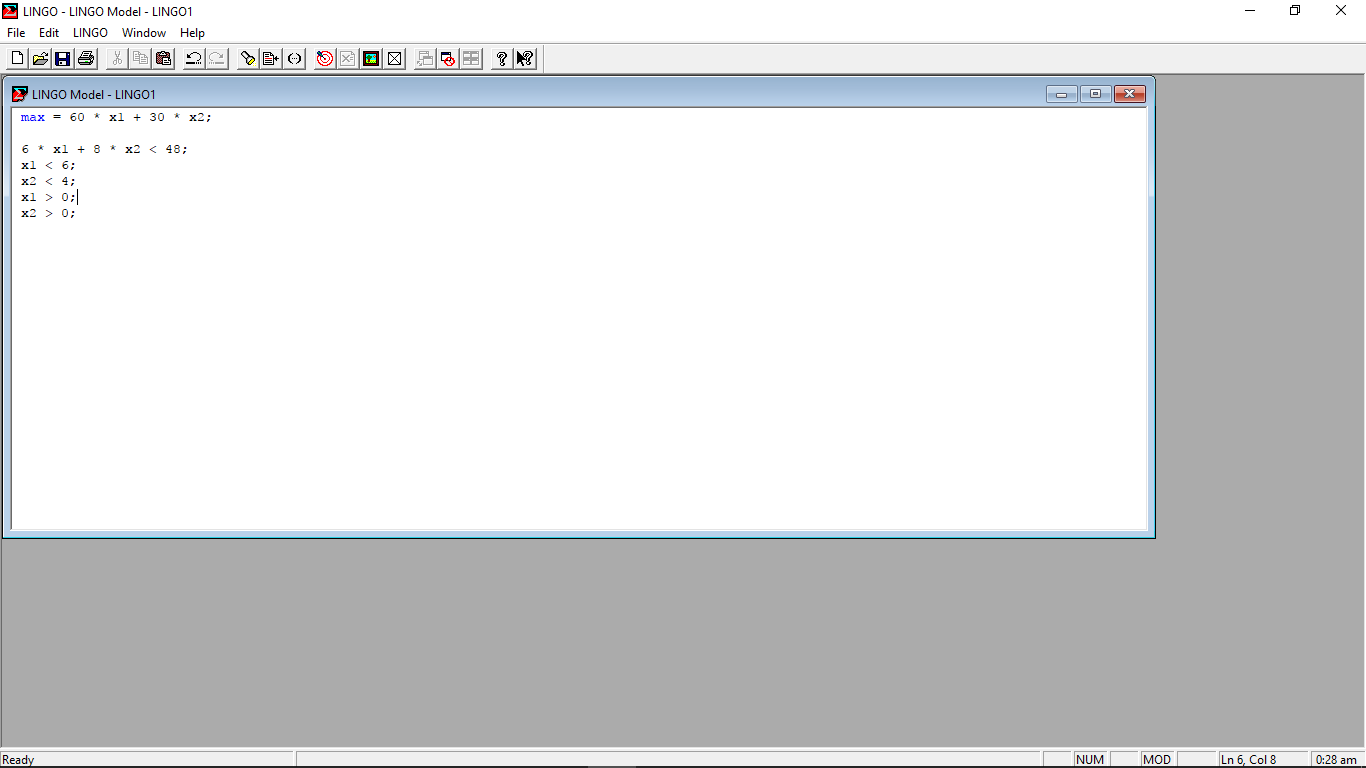
\includegraphics[width=0.9\textwidth]{11}
\end{frame}

\begin{frame}[fragile]{Solución LINGO}
    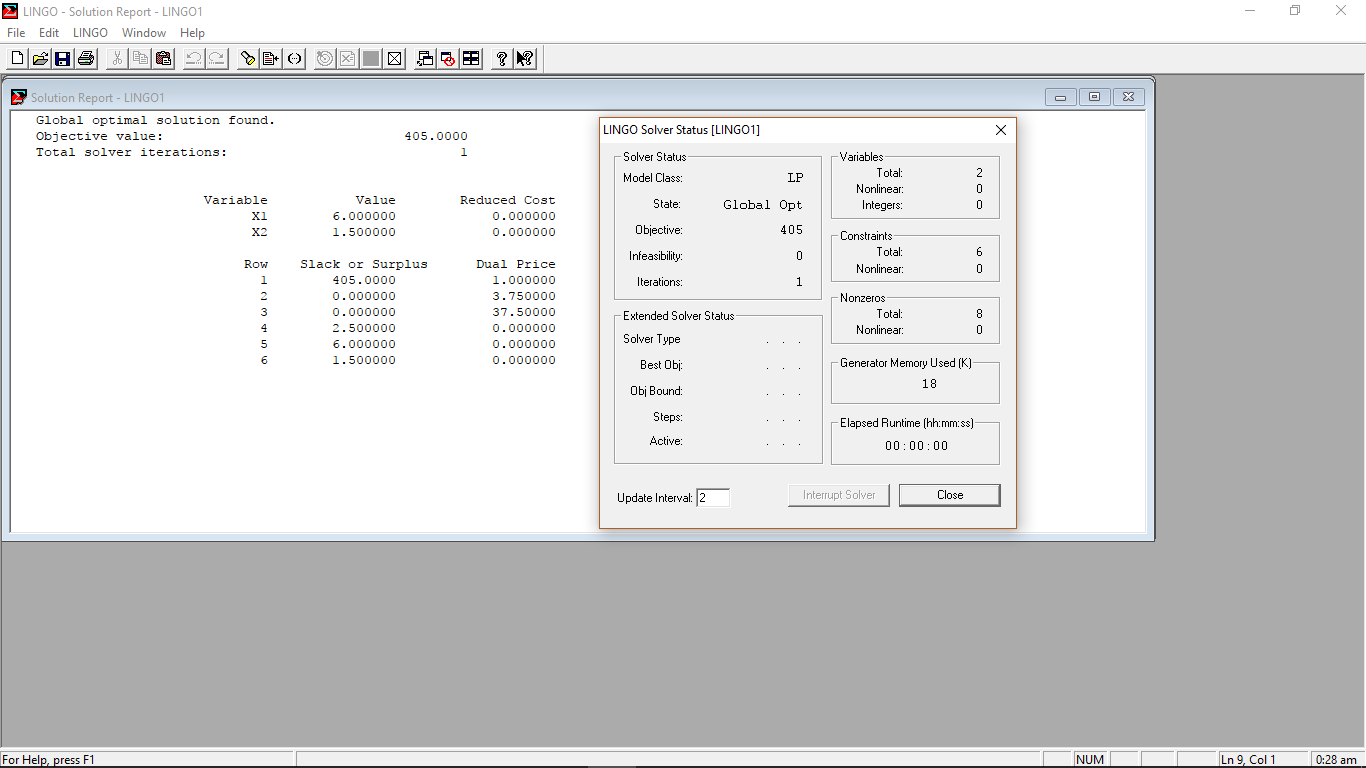
\includegraphics[width=0.9\textwidth]{12}
\end{frame}

\begin{frame}[fragile]{Solución Final}
\[Z = 405.0000\]
\[X_{1} = 6.0000\]
\[X_{2} = 1.5000\]
\end{frame}

%Problema 2
\begin{frame}[t,fragile]{Problema 3.1-7 }
La compañía Word Light produce dos dispositivos para las lámparas (productos 1 y 2) que requieren partes de metal y componentes eléctricas. La administración desea determinar cuántas unidades de cada producto fabricar para maximizar la ganancia. 
\begin{wrapfigure}{c}{0.20\textwidth}
    \centering
    
\includegraphics[width=0.20\textwidth]{2}
\end{wrapfigure}
\end{frame}
\begin{frame}[t,fragile]{Problema 3.1-7 }
Por cada unidad del producto 1 se requieren 1 unidad de partes de metal y 2 unidades de componentes eléctricas, por cada unidad del producto 2 se requieren 3 unidades de partes de metal y 2 unidades de componentes eléctricas, la compañía tiene 200 unidades de partes de metal y 300 de componentes eléctricas, cada unidad del producto 1 da una ganancia de \$ 1 y cada unidad de producto 2, hasta 60 unidades da una ganancia de \$ 2, cualquier exceso de 60 unidades no tiene ganancia por lo que fabricar más de 60 está fuera de consideración. \\
\end{frame}

\begin{frame}[fragile]{Variables de Decisión}
\[P_{1} = producto 1\]
\[P_{2} = producto 2\]

\end{frame}

\begin{frame}[fragile]{Función Objetivo}
Maximizar:\\
\[Z = P_{1} + 2P_{2}\]

\end{frame}

\begin{frame}[fragile]{Restricciones}
\[P_{1} + 3P_{2}  <= 200\]
\[2P_{1} + 2P_{2} <= 300\]
\[P_{2} <= 60\]
\end{frame}

\begin{frame}[fragile]{Modelo Completo}
Maximizar:\\
\[Z = P_{1} + 2P_{2}\]
Sujeto a :\\
\[P1 + 3P2  <= 200\]
\[2P1 + 2P2 <= 300\]
\[P2 <= 60\]
\end{frame}

\begin{frame}[fragile]{Solución LINGO}
    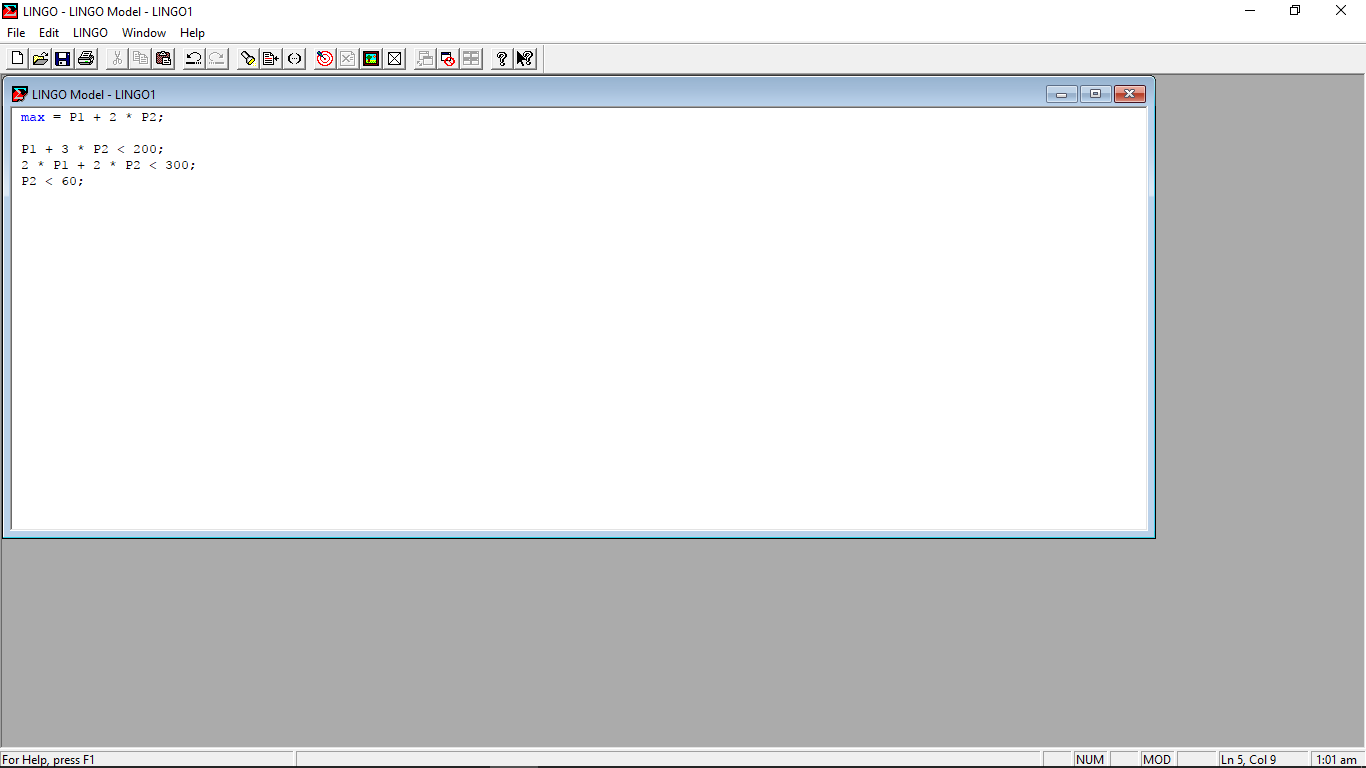
\includegraphics[width=0.9\textwidth]{21}
\end{frame}
\begin{frame}[fragile]{Solución LINGO}
    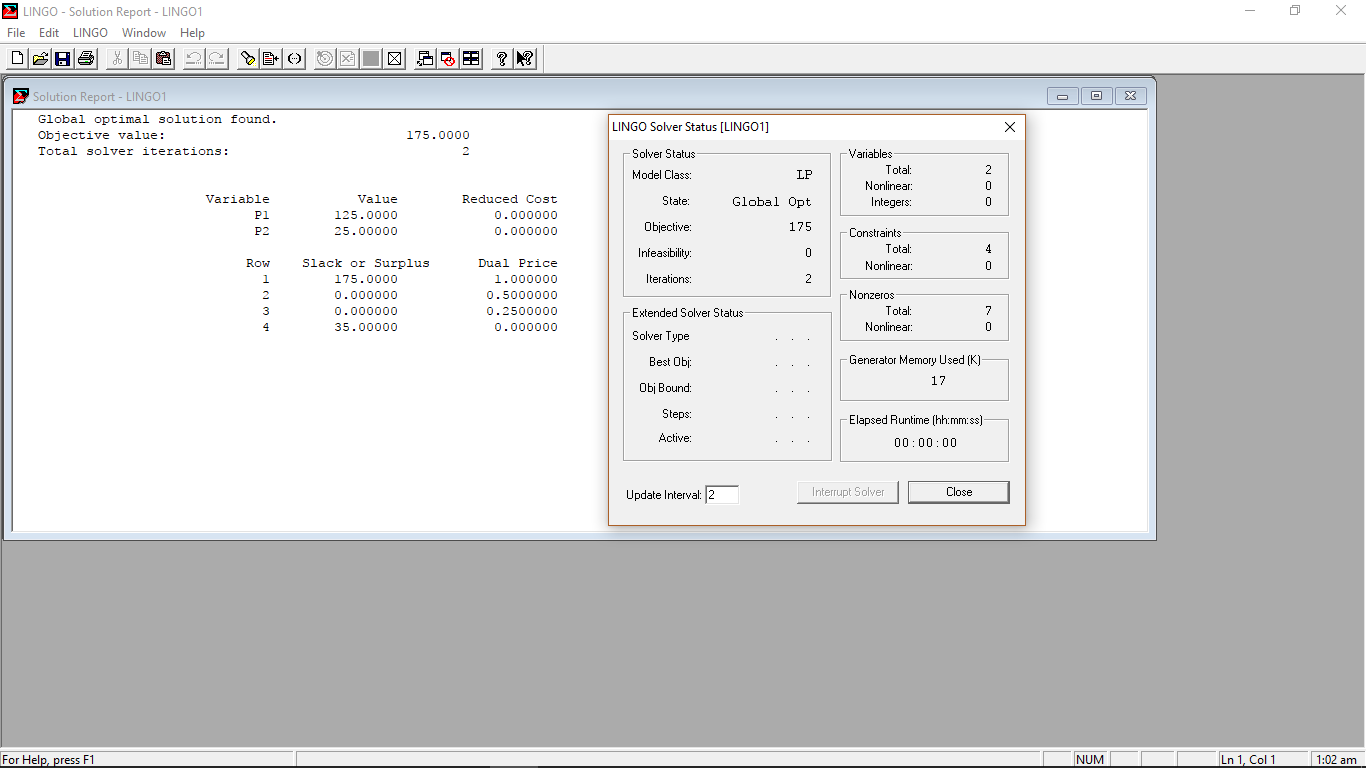
\includegraphics[width=0.9\textwidth]{22}
\end{frame}

\begin{frame}[fragile]{Solución Final}
\[Z = 175.0000\]
\[P_{1} = 125.0000\]
\[P_{2} = 25.0000\]
\end{frame}

%Problema 3
\begin{frame}[t,fragile]{Problema 3.1-8 }
\begin{wrapfigure}{l}{0.20\textwidth}
    \centering
    
\includegraphics[width=0.20\textwidth]{3}
\end{wrapfigure} La compañía de seguros primos está en proceso de introducir dos nuevas líneas de productos: seguro de riesgo especial e hipotecas. La ganancia esperada es \$5 por el seguro de riesgo especial y \$2 por unidad de hipoteca.
La administración debe establecer las cuotas de ventas de las nuevas líneas para maximizar la ganancia total esperada. Los requerimientos de trabajo son los siguientes\\
\end{frame}
\begin{frame}[t,fragile]{Problema 3.1-8 }

\begin{tabular}{|c|c|c|c|}
\hline 
• & \multicolumn{2}{c|}{Horas-hombre por unidad} & Horas-hombre \\ 
\hline 
Deto & Riesgo Especial & Hipoteca & Disponibles \\ 
\hline 
Suscripciones & 3 & 2 & 2400 \\ 
\hline 
Administración & 0 & 1 & 800 \\ 
\hline 
Reclamaciones & 2 & 0 & 1200 \\ 
\hline 
\end{tabular} 
\end{frame}

\begin{frame}[fragile]{Variables de Decisión}
\[X_{1} = seguro de riesgo especial\]
\[X_{2} = hipoteca\]

\end{frame}

\begin{frame}[fragile]{Función Objetivo}
Maximizar:\\
\[Z = 5X_{1} + 2X_{2}\]
\end{frame}

\begin{frame}[fragile]{Restricciones}
\[3X_{1} + 2X_{2} <= 2400\]
\[X_{2} <= 800\]
\[2X_{1} <= 1200\]
\[X_{1}, X_{2} > 0\]

\end{frame}

\begin{frame}[fragile]{Modelo Completo}
Maximizar:\\
\[Z = 5X_{1} + 2X_{2}\]

Sujeto a :\\
\[3X_{1} + 2X_{2} <= 2400\]
\[X_{2} <= 800\]
\[2X_{1} <= 1200\]
\[X_{1}, X_{2} > 0\]
\end{frame}

\begin{frame}[fragile]{Solución LINGO}
    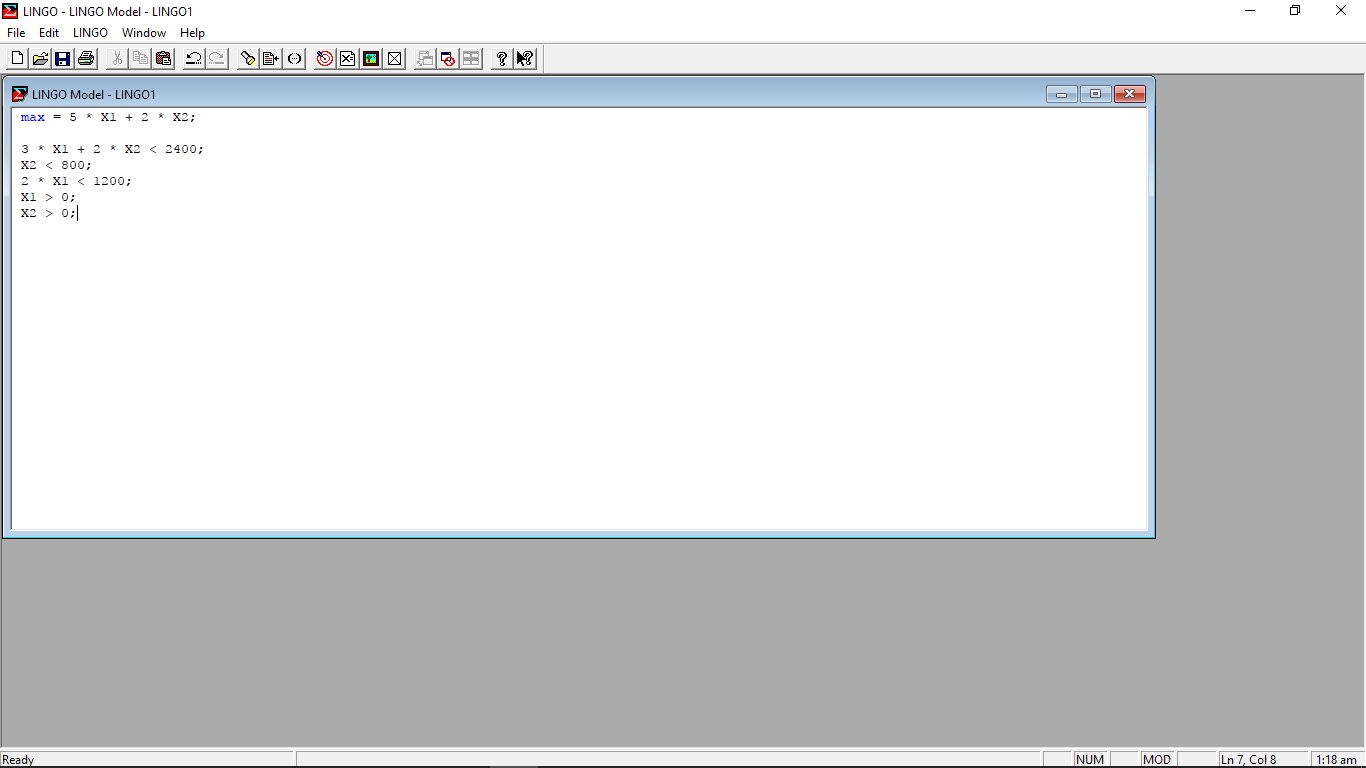
\includegraphics[width=0.9\textwidth]{32}
\end{frame}
\begin{frame}[fragile]{Solución LINGO}
    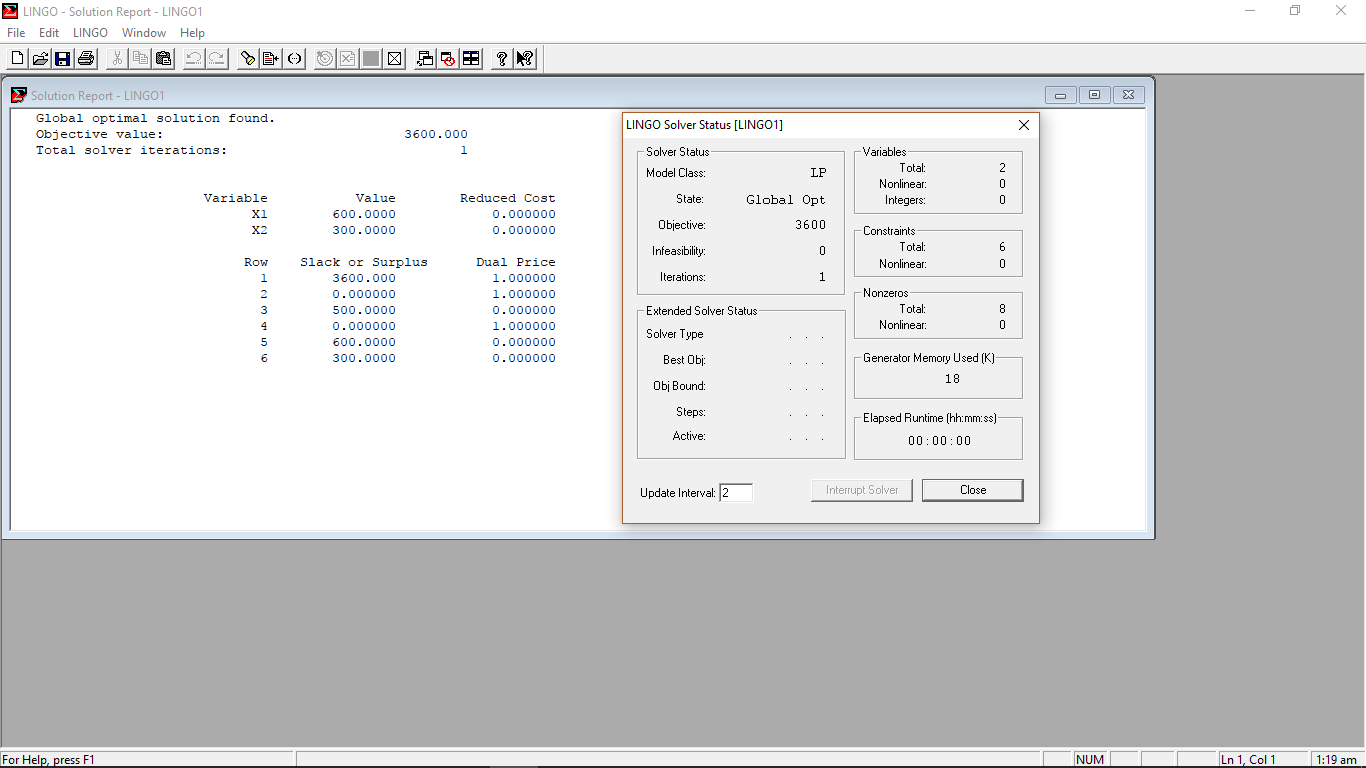
\includegraphics[width=0.9\textwidth]{31}
\end{frame}

\begin{frame}[fragile]{Solución Final}
\[Z = 3 600.0000\]
\[X_{1} = 600.0000\]
\[X_{2} = 300.0000\]
\end{frame}

%Problema 4
\begin{frame}[t,fragile]{Problema  3.1-9}

Weenies and Buns es una planta procesadora de alimentos que fabrica hotdogs y pan para hotdogs. Muelen su propia harina para el pan a una tasa máxima de 200 libras por semana. Cada pan requiere 0.1 libras. Tiene un contrato con Pigland Inc, que especifica la entrega de 800 libras de producto de puerco cada lunes.
\begin{wrapfigure}{r}{0.20\textwidth}
    \centering
    
\includegraphics[width=0.20\textwidth]{4}
\end{wrapfigure}
\end{frame}

\begin{frame}[t,fragile]{Problema  3.1-9}
Cada hotdog requiere 0.25 libras de producto de puerco. Se cuenta con suficiente cantidad del resto de los ingredientes de ambos productos. Por último, la mano de obra consiste en 5 empleados de tiempo completo (40 horas por semana). Cada hotdog requiere 3 minutos de mano de obra y cada pan requiere 2 minutos de mano de obra. Cada hotdog proporciona una ganancia de \$0.20 y cada pan de \$0.10. Weenies and Buns desea saber cuántos hotdogs y cuántos panes deben producir cada semana para lograr la ganancia más alta posible.
\end{frame}
\begin{frame}[fragile]{Variables de Decisión}
\[P = cantidad de panes para hot dog\]
\[H = cantidad de hot dog\]

\end{frame}

\begin{frame}[fragile]{Función Objetivo}
Maximizar:\\
\[Z = 0.2H + 0.1P\]

\end{frame}

\begin{frame}[fragile]{Restricciones}
\[0.1P <= 200\]
\[0.25H <= 800\]
\[2P + 3H <= 1200, y que estamos en minutos, por lo tanto son 5 empleados que trabajan 40 horas por semana, lo cual es 2400 minutos, ahora son 5, por lo tanto hay disponible 12 000 minutos.\]

\end{frame}

\begin{frame}[fragile]{Modelo Completo}
Maximizar:\\
 \[Z = 0.2H + 0.1P\]
sujeto a:\\
\[0.1P <= 200\]
\[0.25H <= 800\]
\[2P + 3H <= 1200, y que estamos en minutos, por lo tanto son 5 empleados que trabajan 40 horas por semana, lo cual es 2400 minutos, ahora son 5, por lo tanto hay disponible 12 000 minutos.\]
\end{frame}

\begin{frame}[fragile]{Solución LINGO}
    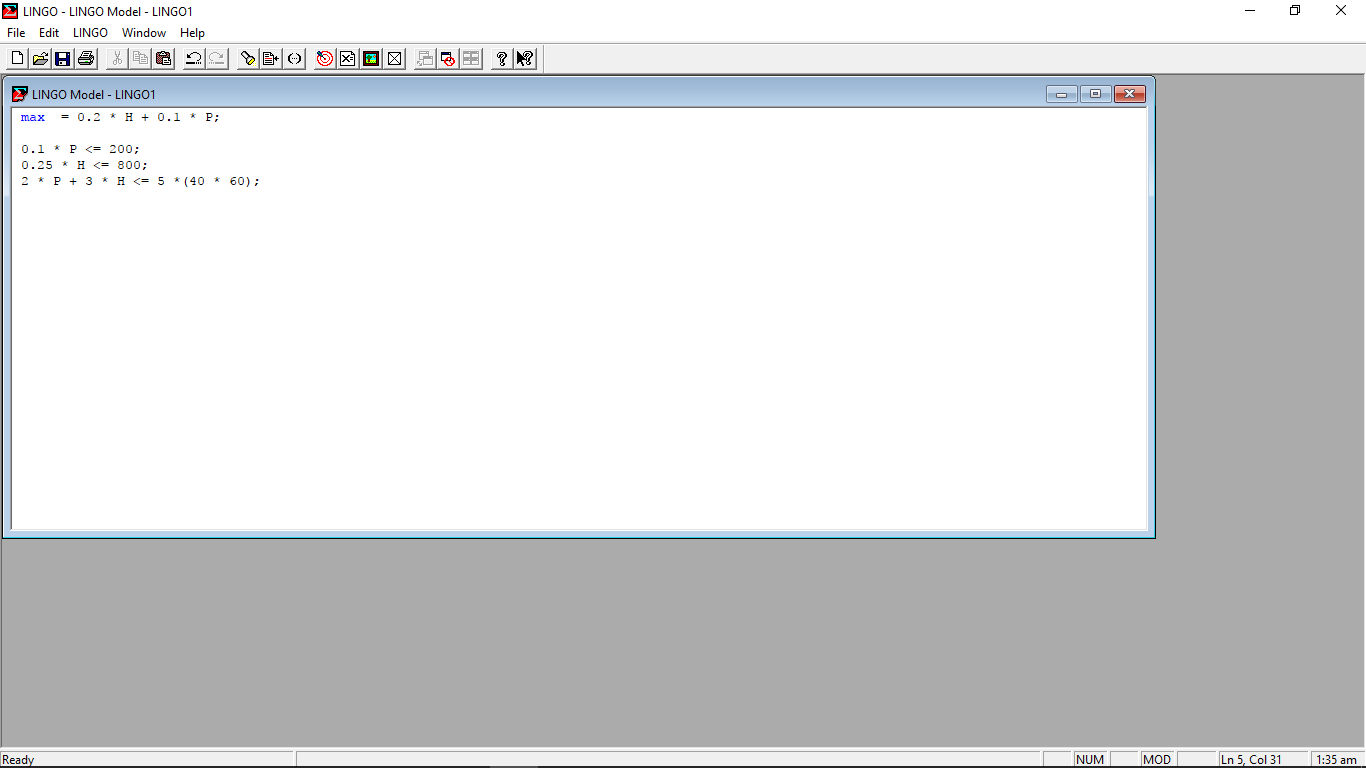
\includegraphics[width=0.9\textwidth]{42.png}
\end{frame}
\begin{frame}[fragile]{Solución LINGO}
    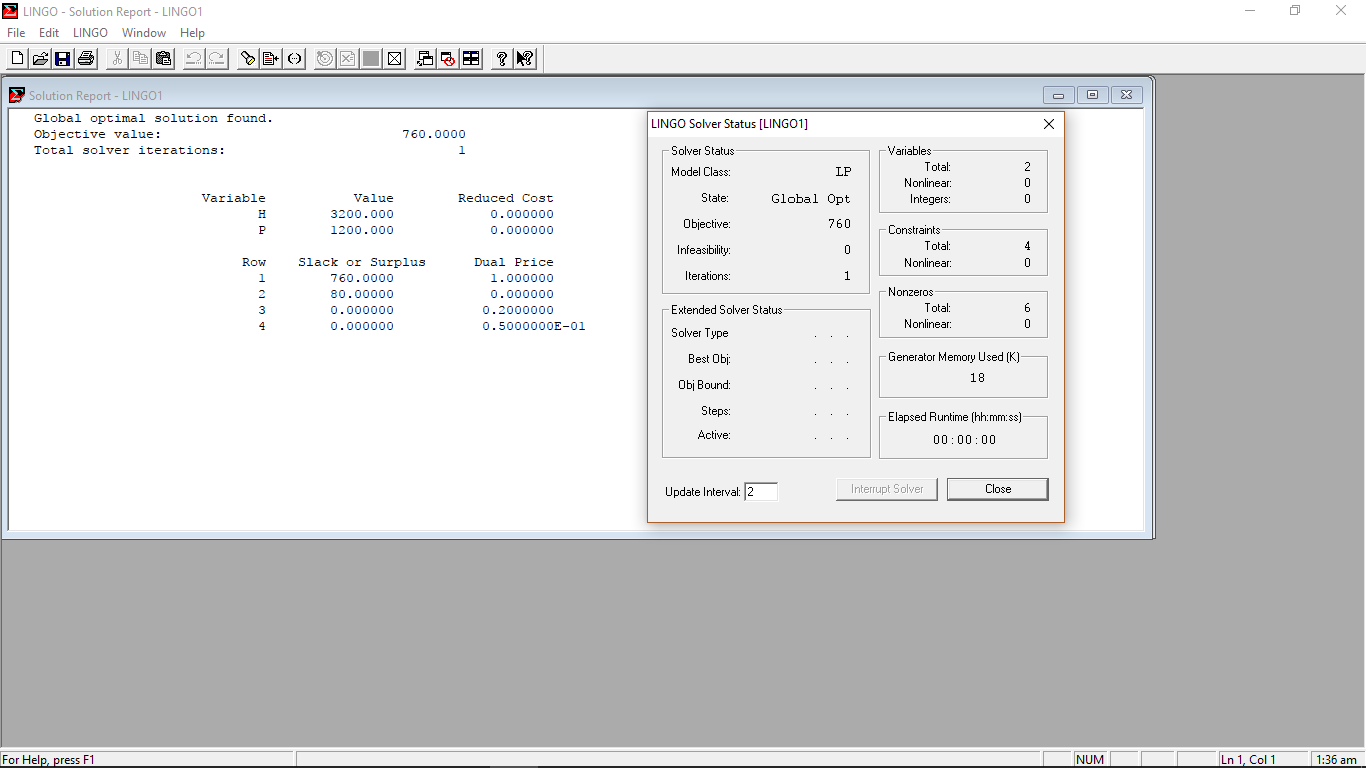
\includegraphics[width=0.9\textwidth]{41.png}
\end{frame}

\begin{frame}[fragile]{Solución Final}
\[Z = 760.0000\]
\[H = 3 200.0000\]
\[P = 1 200.0000\]
\end{frame}

%Problema 5
\begin{frame}[t,fragile]{Problema 3.2-3}
Hoy es un día de suerte. Acaba de ganar un premio de \$10.000. Dedicara \$4.000 a impuestos y diversiones, pero ha decidido invertir los otros \$6.000. \begin{wrapfigure}{r}{0.20\textwidth}
    \centering
    
\includegraphics[width=0.20\textwidth]{5}
\end{wrapfigure}Al oír las nuevas, dos amigos le han ofrecido una oportunidad de convertirse en socio en dos empresas distintas, cada una planeada por cada uno de ellos. En ambos casos, la inversión incluye dedicar parte de su tiempo el siguiente verano y dinero en efectivo. Para ser un socio completo en el caso del primer amigo debe invertir \$ 5000 y 400 horas, y su ganancia estimada (sin tomar en cuenta el valor del dinero en el tiempo) seria \$ 450. 

\end{frame}
\begin{frame}[t,fragile]{Problema  3.1-9}
Las cifras correspondientes para el segundo caso son \$ 4000 y 500 horas, con una ganancia estima de \$ 4500. Sin embargo, ambos amigos son flexibles y le permitirían participar con cualquier fracción de participación que quiera. Si elige una participación parcial, todas las cifras dadas para sociedad completa (inversión de dinero y tiempo, y la ganancia) se pueden multiplicar por esta fracción. \\
Como de todas formas usted busca un trabajo de verano interesante (máximo 600 horas), a decidido participar en una o ambas empresas en alguna combinación que maximice su ganancia total estimada. Usted debe resolver el problema de encontrar la mejor combinación.
\end{frame}

\begin{frame}[fragile]{Variables de Decisión}
\[P_{1} = participación Amigo 1\]
\[P_{2} = participación Amigo 2\]

\end{frame}

\begin{frame}[fragile]{Función Objetivo}
Maximizar\\
\[Z = 4500P_{1} + 4500P_{2}\]

\end{frame}

\begin{frame}[fragile]{Restricciones}
\[5000P_{1} + 4000P_{2} <= 6000 inversión total\]
\[400P_{1} + 5000P_{2} <= 600 horas disponible\]
\[P_{1}, P_{2} > 0\]

\end{frame}

\begin{frame}[fragile]{Modelo Completo}
Maximizar\\
\[Z = 4500P_{1} + 4500P_{2}\]

Sujeto a:\\
\[5000P_{1} + 4000P_{2} <= 6000 inversión total\]
\[400P_{1} + 5000P_{2} <= 600 horas disponible\]
\[P_{1}, P_{2} > 0\]

\end{frame}

\begin{frame}[fragile]{Solución LINGO}
    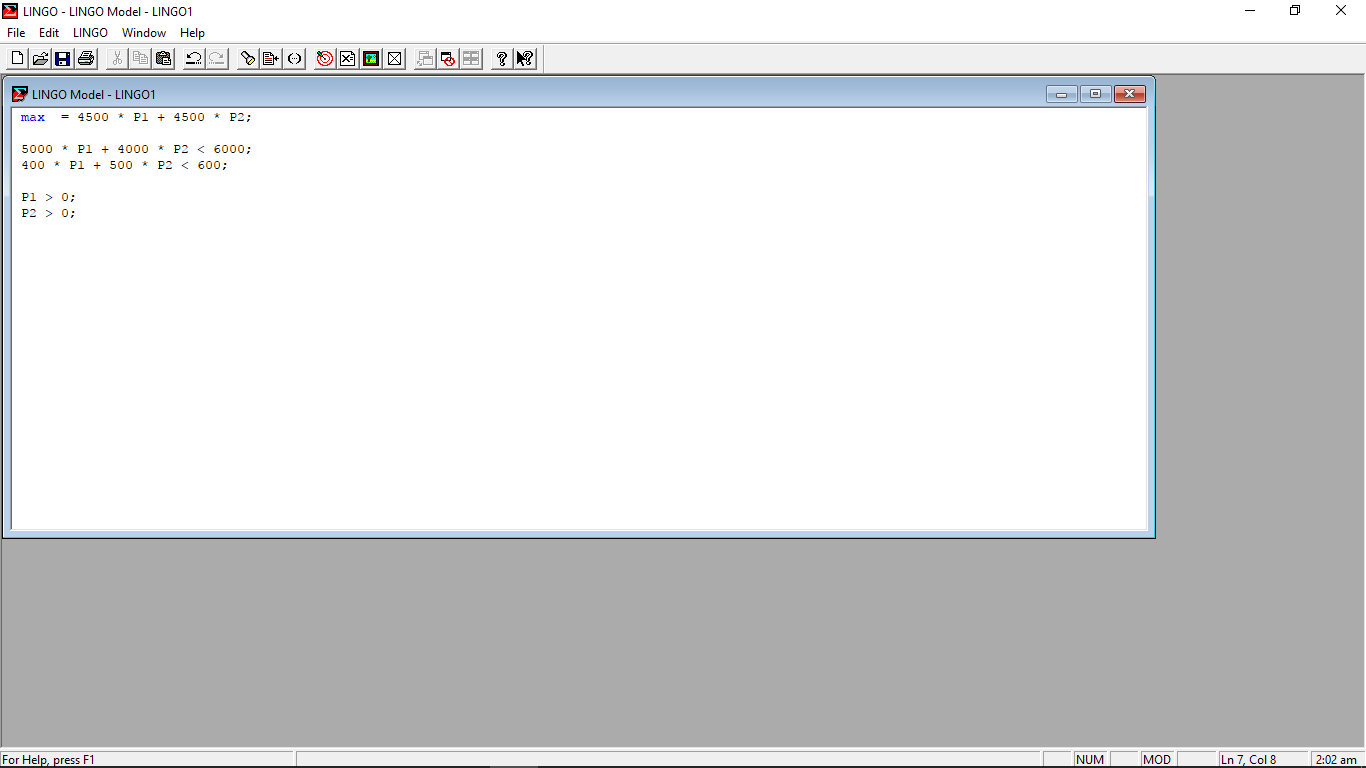
\includegraphics[width=0.9\textwidth]{51.png}
\end{frame}
\begin{frame}[fragile]{Solución LINGO}
    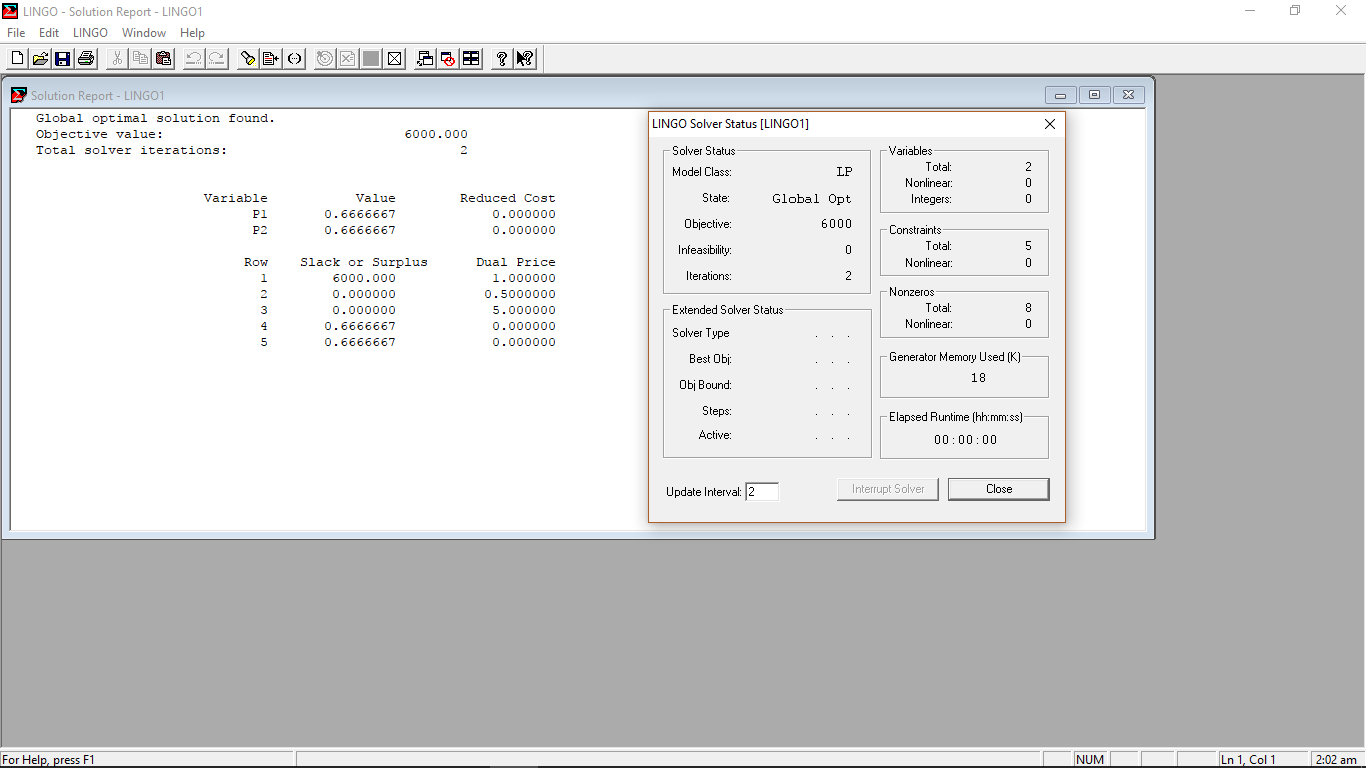
\includegraphics[width=0.9\textwidth]{52.png}
\end{frame}

\begin{frame}[fragile]{Solución Final}
\[Z = 6 000.0000\]
\[P_{1} = 0.6666667\]
\[P_{2} = 0.6666667\]
\end{frame}

%Problema 6
\begin{frame}[t,fragile]{Problema 3.4-7}
La carne con papas es el plato favorito de Ralph Edmund. Por eso decidió hacer dieta continua de sólo estos dos alimentos (más algunos líquidos y suplementos de vitaminas) en todas las comidas. Ralph sabe que ésa no es la dieta más sana y quiere asegurarse de que toma cantidades adecuadas de  los dos alimentos para satisfacer los requerimientos nutricionales. Cuenta con la siguiente información.\begin{wrapfigure}{c}{0.20\textwidth}
    \centering
    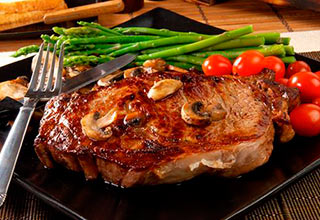
\includegraphics[width=0.20\textwidth]{6}
\end{wrapfigure}
\end{frame}
\begin{frame}[t,fragile]{Problema 3.4-7}

\begin{tabular}{|c|c|c|c|}
\hline 
Ingrediente & Gramos por porción &   & Requerimientos diarios\\ 
\hline 
  & Res & Papa &   \\ 
\hline 
Carboidratos & 5 & 15 & >= 50 \\ 
\hline 
Proteínas & 20 & 5 & >= 40 \\ 
\hline 
Grasa & 15 & 2 & <= 60 \\ 
\hline 
Costo Por Porción & \$14 & \$2 & • \\ 
\hline 
\end{tabular} \\
Ralph requiere determinar el número de porciones diarias (pueden ser fraccionarias) de res y  papas que cumplirían con estos requerimientos a un costo mínimo.
\end{frame}

\begin{frame}[fragile]{Variables de Decisión}
\[x_{1} = Gramos por porción de Res\]
\[x_{2} = Gramos por porción de Papa\]

\end{frame}

\begin{frame}[fragile]{Función Objetivo}
Minimizar\\
\[Z = 4x_{1} + 2x_{2}\]

\end{frame}

\begin{frame}[fragile]{Restricciones}
\[5x_{1} + 15x_{2} >= 50\]
\[20x_{1} +5x_{2} >= 40\]
\[15x_{1} + 2x_{2} <=60\]
\[x_{1} , x_{2} >= 0\]

\end{frame}

\begin{frame}[fragile]{Modelo Completo}
Minimizar\\
\[Z = 4x_{1} + 2x_{2}\]
Sujeto a :\\
\[5x_{1} + 15x_{2} >= 50\]
\[20x_{1} +5x_{2} >= 40\]
\[15x_{1} + 2x_{2} <= 60\]
\[x_{1}, >= 0\]
\end{frame}

\begin{frame}[fragile]{Solución LINGO}
    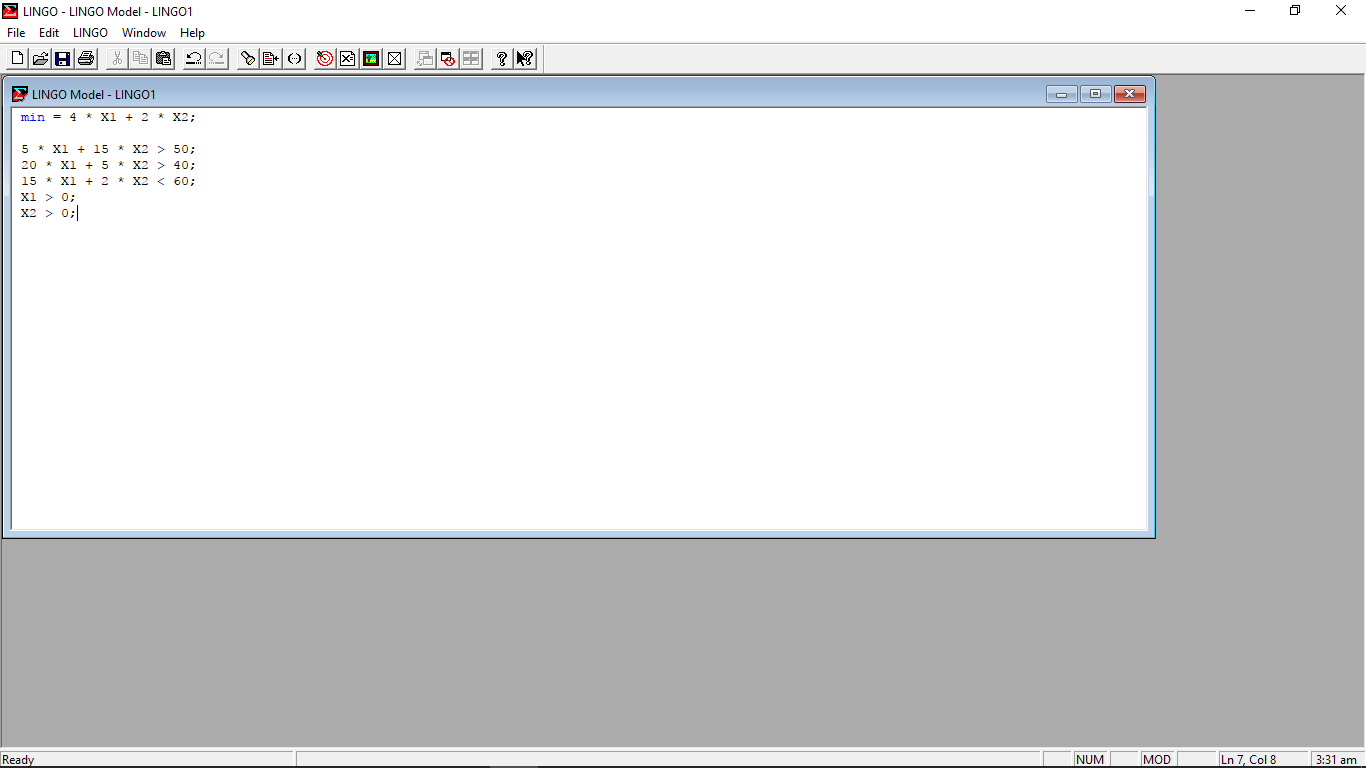
\includegraphics[width=0.9\textwidth]{61.png}
\end{frame}
\begin{frame}[fragile]{Solución LINGO}
    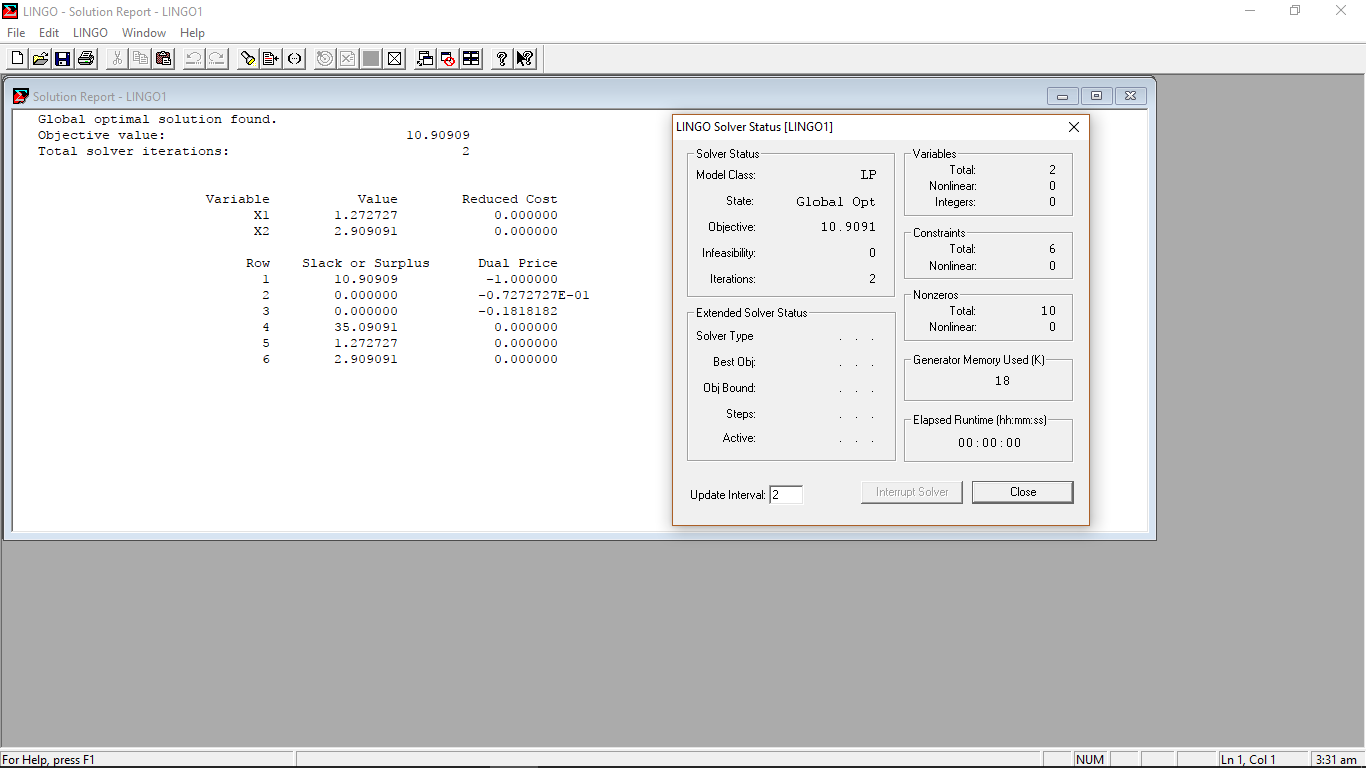
\includegraphics[width=0.9\textwidth]{63.png}
\end{frame}

\begin{frame}[fragile]{Solución Final}
\[Z = 10.90909\]
\[X_{1} = 1.2727\]
\[X_{2} = 2.909091\]
\end{frame}

%Problema 7
\begin{frame}[t,fragile]{Problema 3.4-8 }
Web Mercantile vende muchos productos para el hogar mediante un catálogo en línea. La compañía  necesita un gran espacio para almacenar los productos. En la actualidad planea rentar espacio para los siguientes 5 meses. Se sabe cuánto espacio necesitará cada mes, pero como el mismo varía mucho, puede ser más económico rentar sólo la cantidad  de necesaria cada mes con contratos mensuales.
\begin{wrapfigure}{c}{0.20\textwidth}
    \centering
    
\includegraphics[width=0.20\textwidth]{7}
\end{wrapfigure}
\end{frame}
\begin{frame}[t,fragile]{Problema 3.4-7}
Por otro lado, el costo adicional de rentar espacio para meses adicionales es menor que para el primero, y puede ser menos costoso rentar el espacio máximo lo 5 meses. Otra opción es el enfoque intermedio de cambiar la cantidad total de  espacio rentado (con un nuevo contrato y/o terminación del anterior) al menos una vez pero no cada mes.
\end{frame}

\begin{frame}[t,fragile]{Problema 3.4-8 }
El espacio requerido si los costos de arrendamiento son los siguientes:
\begin{tabular}{|c|c|c|c|}
\hline 
Mes & Espacio Requerido & Periodo & Costo por ft^2 arrendado \\ 
\hline 
1 & 30000 & 1 & \$65 \\ 
\hline 
2 & 20000 & 2 & \$100 \\ 
\hline 
3 & 40000 & 3 & \$135 \\ 
\hline 
4 & 10000 & 4 & \$160 \\ 
\hline 
5 & 50000 & 5 & \$190 \\ 
\hline 
\end{tabular} \\
El objetivo es minimizar el costo total de arrendamiento para cumplir con los requerimientos.
\end{frame}

\begin{frame}[fragile]{Análisis}
Debemos pensar en los .meses que vamos a arrendar, podemos arrendar el espacio máximo por los cinco meses, esto permite inferir que debemos alquilar al menos el espacio indicado en la tabla del problema. Además tenemos que considerar o clasificar los meses que afectan cada uno de los contratos.

\end{frame}
\begin{frame}[fragile]{Variables de Decisión}
\(A_{1}\) = Espacio a arrendar el primer mes por el periodo de 1 mes\\
\(A_{2}\) = Espacio a arrendar el primer mes por el periodo de 2 meses\\
\(A_{3}\) = Espacio a arrendar el primer mes por el periodo de 3 meses\\
\(A_{4}\) = Espacio a arrendar el primer mes por el periodo de 4 meses\\
\(A_{5}\) = Espacio a arrendar el primer mes por el periodo de 5 meses\\
\(B_{1}\) = Espacio a arrendar el segundo mes por el periodo de 1 mes\\
\(B_{2}\) = Espacio a arrendar el segundo mes por el periodo de 2 meses\\
\(B_{3}\) = Espacio a arrendar el segundo mes por el periodo de 3 meses\\
\(B_{4}\) = Espacio a arrendar el segundo mes por el periodo de 4 meses\\
\(B_{5}\) = No tiene sentido, no se puede\\
\(C_{1}\) = Espacio a arrendar el tercer mes por el periodo de 1 mes\\
\(C_{2}\) = Espacio a arrendar el tercer mes por el periodo de 2 meses\\
\(C_{3}\) = Espacio a arrendar el tercer mes por el periodo de 3 meses\\
\(C_{4}\) y C5 =  No tiene sentido, no se puede.\\
\(D_{1}\) = Espacio a arrendar el cuarto mes por el periodo de 1 mes\\
\(D_{2}\) = Espacio a arrendar el cuarto mes por el periodo de 2 meses\\
\(D_{3}, D_{4} y D_{5}\) =  No tiene sentido, no se puede.\\
\(E_{1}\) = Espacio a arrendar el quinto mes por el periodo de 1 mes\\
\(E_{2} , E_{3}, E_{4}, E_{5}\) =  No tiene sentido, no se puede.\\

\end{frame}

\begin{frame}[fragile]{Función Objetivo}
Minimizar\\
\[Z = 65 A_{1} + 100 A_{2} + 135 A_{3} + 160 A_{4} + 190 A_{5} + 65 B_{1} + 100 B_{2} + 135 B_{3} + 160 B_{4} + 65 C_{1} + 100 C_{2} + 135 C_{3} + 65 D_{1} + 100 D_{2} + 65 E_{1}\]

\end{frame}

\begin{frame}[fragile]{Restricciones}
\[MES 1: A_{1} + A_{2} + A_{3} + A_{4} + A_{5} >= 30.000 \]
\[MES 2: A_{2} + A_{3} + A_{4} + A_{5} + B_{1} + B_{2} + B_{3} + B_{4} >= 20.000 \]
\[MES 3: A_{3} + A_{4} + A_{5} + B_{2} + B_{3} + B_{4} + C_{1} + C_{2} + C_{3} >= 40.000 \]
\[MES 4: A_{4} + A_{5} + B_{3} + B_{4} + C_{2} + C_{3} + D_{1} + D_{2} >= 10.000\]
\[MES 5: A_{5} + B_{4}  + C_{3} + D_{2} + E_{1} = 50.000\]

\end{frame}

\begin{frame}[fragile]{Modelo Completo}
Minimizar\\
\[Z = 65 A_{1} + 100 A_{2} + 135 A_{3} + 160 A_{4} + 190 A_{5} + 65 B_{1} + 100 B_{2} + 135 B_{3} + 160 B_{4} + 65 C_{1} + 100 C_{2} + 135 C_{3} + 65 D_{1} + 100 D_{2} + 65 E_{1}\]
Sujeto a :\\
\[A_{1} + A_{2} + A_{3} + A_{4} + A_{5} >= 30.000 \]
\[A_{2} + A_{3} + A_{4} + A_{5} + B_{1} + B_{2} + B_{3} + B_{4} >= 20.000 \]
\[A_{3} + A_{4} + A_{5} + B_{2} + B_{3} + B_{4} + C_{1} + C_{2} + C_{3} >= 40.000 \]
\[A_{4} + A_{5} + B_{3} + B_{4} + C_{2} + C_{3} + D_{1} + D_{2} >= 10.000\]
\[A_{5} + B_{4}  + C_{3} + D_{2} +E_{1} = 50.000\]

\end{frame}

\begin{frame}[fragile]{Solución LINGO}
    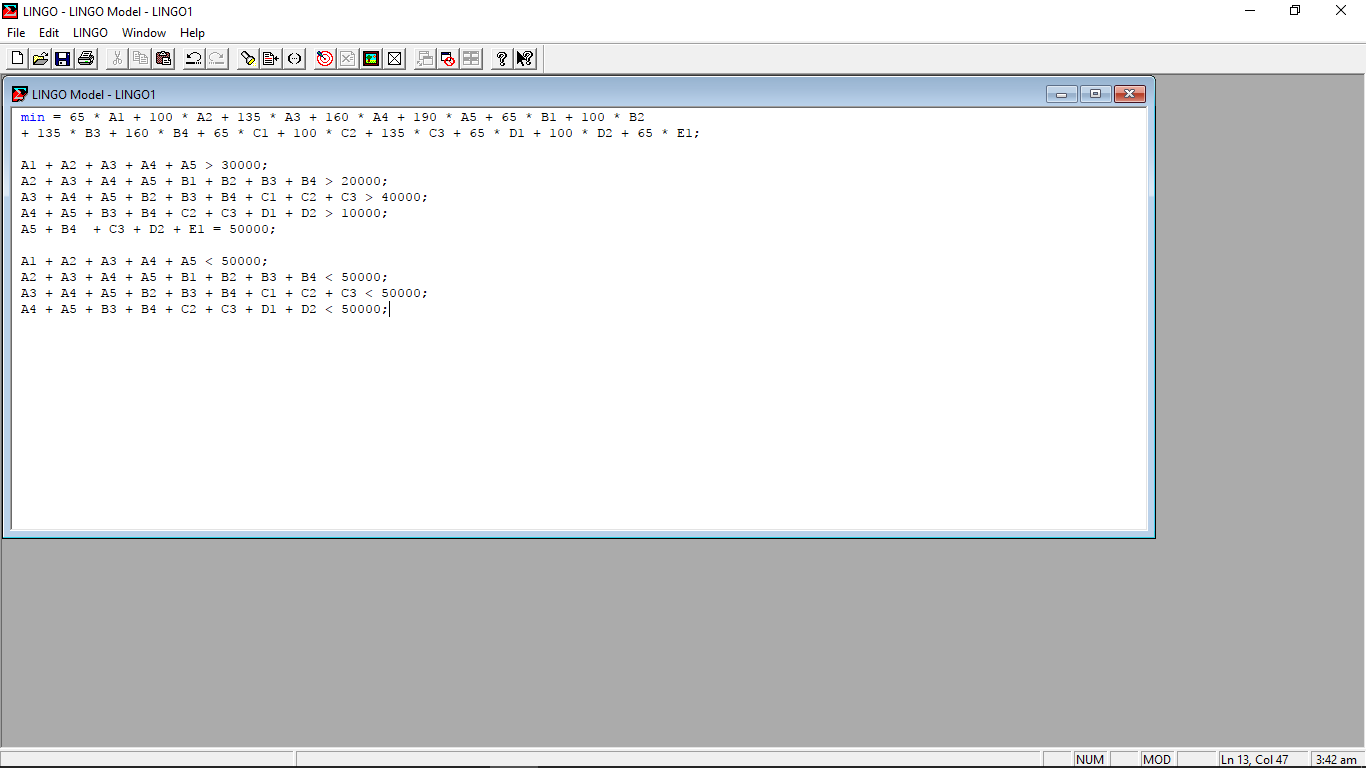
\includegraphics[width=0.9\textwidth]{72}
\end{frame}
\begin{frame}[fragile]{Solución LINGO}
    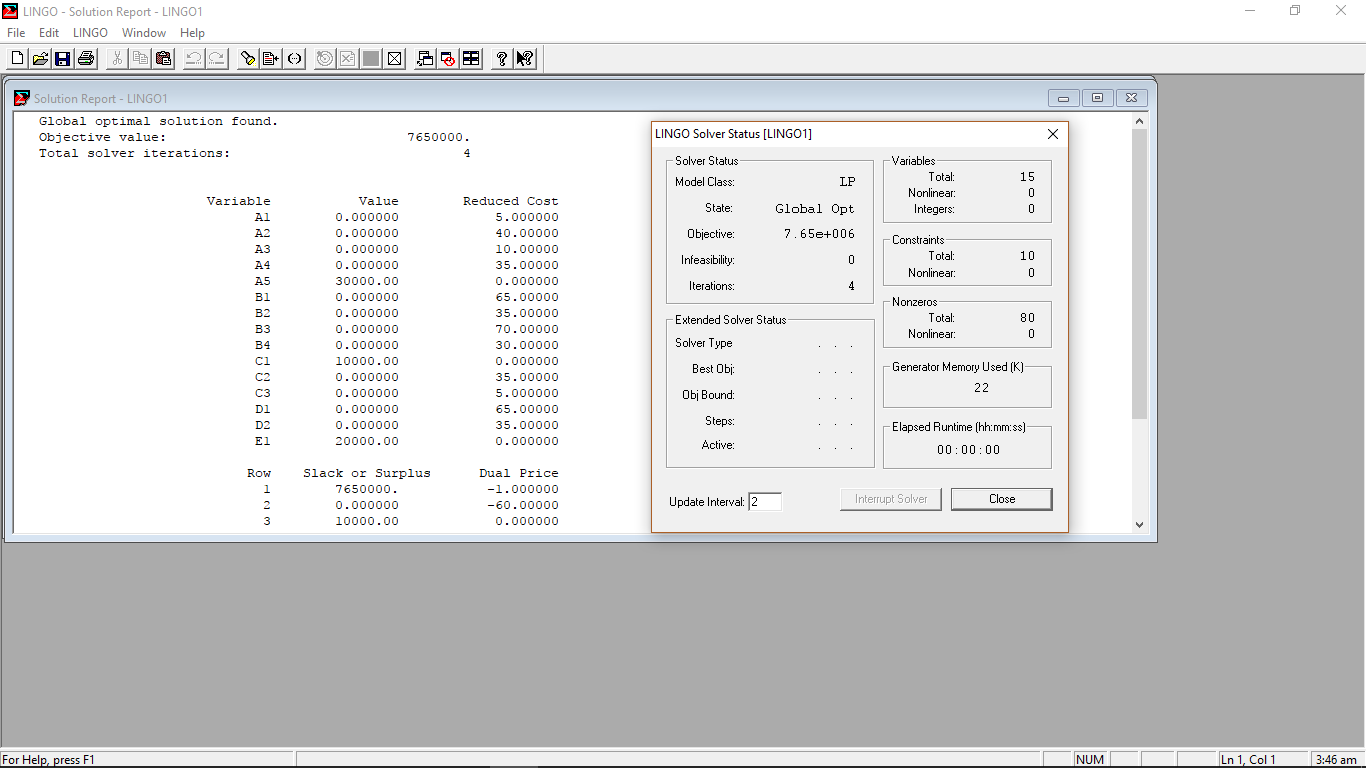
\includegraphics[width=0.9\textwidth]{71}
\end{frame}

\begin{frame}[fragile]{Solución Final}
\[Z = 7650000\]
\[A_{1} = 0.0000\]
\[A_{2} = 0.0000\]
\[A_{3} = 0.0000\]
\[A_{4} = 0.0000\]
\[A_{5} = 30 000.00\]
\[B_{1} = 0.0000\]
\[B_{2} = 0.0000\]
\[B_{3} = 0.0000\]
\[B_{4} = 0.0000\]
\[C_{1} = 10 000.00\]
\[C_{2} = 0.0000\]
\[C_{3} = 0.0000\]
\[D_{1} = 0.0000\]
\[D_{2} = 0.0000\]
\[E_{1} = 20 000.00\]

\end{frame}

%Problema 8
\begin{frame}[t,fragile]{Problema 3.4-14 }
Oxbridge University tiene una computadora grande para uso de académicos, estudiantes de doctorado y ayudantes de investigación. Durante las horas hábiles debe haber un trabajador para operador y dar mantenimiento a la computadora y realizar algunos servicios  de programación. Beryl Ingram, director del centro de cómputo, coordina la operación.
\begin{wrapfigure}{c}{0.20\textwidth}
    \centering
    
\includegraphics[width=0.20\textwidth]{8}
\end{wrapfigure}
\end{frame}
\begin{frame}[t,fragile]{Problema 3.4-14 }
Al principio del semestre de  otoño , Beryl se enfrenta al problema de asignar horas de trabajo distintas a sus operadores. Debido a que éstos son estudiantes de la universidad, están disponibles para el trabajo solo un número limitado de horas al dia, como se muestra en la tabla. \\

\begin{tabular}{|c|c|c|c|c|c|c|}
\hline 
• & • & \multicolumn{5}{c|}{Máximo de horas disponibles} \\ 
\hline 
Operador & Salarios & Lun. & Mar. & Mié. & Jue. & Vie. \\ 
\hline 
K.C. & \$10.00/hora & 6 & 0 & 6 & 0 & 6 \\ 
\hline 
D.H. & \$10.10/hora & 0 & 6 & 0 & 6 & 0 \\ 
\hline 
H.B. & \$9.90/hora & 4 & 8 & 4 & 0 & 4 \\ 
\hline 
S.C. & \$9.80/hora & 5 & 5 & 5 & 0 & 5 \\ 
\hline 
K.S. & \$10.80/hora & 3 & 0 & 3 & 8 & 0 \\ 
\hline 
N.K. & \$11.30/hora & 0 & 0 & 0 & 6 & 2 \\ 
\hline 
\end{tabular} 
\end{frame}
\begin{frame}[t,fragile]{Problema 3.4-14 }
Hay seis operadores (cuatro de licenciatura y dos de posgrado). Todos tienen salarios diferentes según su experiencia con computadoras y su aptitud para programar. La tabla muestra estos salarios junto con el número máximo de horas al día que cada uno puede trabajar.\\
Se garantiza a cada operador un número mínimo de horas de trabajo a la semana que lo mantendrán con un conocimiento adecuado de la operación. Este nivel se estableció de modo arbitrario en 8 horas por semana para licenciatura (K.C., D.H., H.B. y S.C.) y 7 horas por semana para posgrado (K.S. y N.K.).\\
\end{frame}
\begin{frame}[t,fragile]{Problema 3.4-14 }
El centro de computo debe abrir de 8 am a 10 pm de lunes a viernes con un operador de guardia en este horario. Sábados y domingos, otras personas lo operan. Debido al presupuesto reducido, Beryl tiene que minimizar el costo. Ella quiere determinar el número de horas que debe asignar a cada operador cada día. \begin{wrapfigure}{r}{0.20\textwidth}
    \centering
    
\includegraphics[width=0.20\textwidth]{8}
\end{wrapfigure}

\end{frame}
\begin{frame}{Análisis}
Se requiere minimizar el costo  de las horas de cada operador en cada día. 
Para ello, podemos ver como una “matriz” \(X_{ij}\), donde  i es cada operador, y j es el día de la semana (i = KC, DH, HB, SC, KS, NK;  j = lu, ma, mi, ju, vi).
Z = costo (salario * tiempo max disponible por trabajador * horas asignadas)

\end{frame}

\begin{frame}[fragile]{Variables de Decisión}
\[x_{11} =  Horas asignadas al operador KC el lunes\]
\[x_{12} = Horas asignadas al operador KC el martes\]
\[x_{13} =  Horas asignadas al operador KC el miércoles\]
\[x_{14}   = Horas asignadas al operador KC el jueves\]
\[x_{15} =  Horas asignadas al operador KC el viernes\]
\end{frame}
\begin{frame}[fragile]{Variables de Decisión}
Lo mismo para  el operador 2 DH\\
\[x_{21} =  Horas asignadas al operador DH el lunes\]
\[x_{22} = Horas asignadas al operador DH el martes\]
\[x_{23} =  Horas asignadas al operador DH el miércoles\]
\[x_{24} = Horas asignadas al operador DH el jueves\]
\[x_{25} =  Horas asignadas al operador DH el viernes\]

...\\
\[Lo mismo para el operador 6 NK\]
\[X_{61} =  Horas asignadas al operador NK el lunes\]
\[X_{62} = Horas asignadas al operador NK el martes\]
\[X_{63} =  Horas asignadas al operador NK el miércoles\]
\[X_{64} = Horas asignadas al operador NK el jueves\]
\[X_{65} =  Horas asignadas al operador NK el viernes\]


\end{frame}

\begin{frame}[fragile]{Función Objetivo}
Minimizar
\[Z = 10.00 (x_{11} + x_{12} +x_{13}+x_{14} +x_{15}) \]
\[+ 10.10 (x_{21} + x_{22} +x_{23}+x_{24} + x_{25})\]
\[+  9.90 (X_{31} + X_{32} +X_{33}+X_{34} +X_{35})\]
\[+ 9.80  (X_{41} + X_{42} +X_{43}+X_{44} +X_{45})\]
\[+ 10.80  (X_{51} + X_{52} +X_{53}+X_{54} +X_{55})\]
\[+ 11.30  (X_{61} + X_{62} +X_{63}+X_{64} +X_{65}\]

\end{frame}

\begin{frame}[fragile]{Restricciones}
/* Restricciones  de mínimo número de horas a la semana K.C., D.H., H.B. y S.C. = 8, K.S. y N.K. = 7. */\\
\[x_{1}1 + x_{12} +x_{1}3+x_{1}4 +x_{1}5 >=8\]
\[x_{2}1 + x_{22} +x_{2}3+x_{2}4 + x_{2}5 >= 8\]
\[X_{31} + X_{32} +X_{33}+X_{34} +X_{35} >= 8\]
\[X_{41} + X_{42} +X_{43}+X_{44} +X_{45} >= 8\]
\[X_{51} + X_{52} +X_{53}+X_{54} +X_{55} >= 7\]
\[X_{61} + X_{62} +X_{63}+X_{64} +X_{65} >= 7\]
\end{frame}
\begin{frame}[fragile]{Restricciones}
/* El centro de cómputo abre de 8 am hasta 10 pm  (14 horas), donde siempre hay un operador, esto para toda la semana*/\\
\[Lunes => x_{11} + x_{21} + X_{31} +X_{41} + X_{51} +X_{61} = 14  \]
\[Martes=> x_{12} + x_{22} + X_{32} +X_{42} + X_{52} + X_{62} = 14\]
\[Miercoles=> x_{13} + x_{23} + X_{33} +X_{43} + X_{53} +X_{63} = 14\]
\[Jueves => x_{14} + x_{24} + X_{34} +X_{44} + X_{54} +X_{64} = 14\]
\[Viernes => x_{15} + x_{25} + X_{35} +X_{45} + X_{55} +X_{65} = 14  \]

\end{frame}
\begin{frame}[fragile]{Restricciones}
/* Horas disponibles por día, para cada trabajador*/\\
Operador 1\\
    \[x_{11} <= 6\]
    \[x_{12} = 0\]
    \[x_{13} <= 6\]
    \[x_{14}  = 0\]
    \[x_{15} <= 6\]
Operador 2\\
    \[x_{21} = 0 \]
    \[x_{22} <= 6\]
    \[x_{23} = 0\]
    \[x_{24}  <= 6\]
    \[x_{25} = 0\]
\end{frame}
\begin{frame}[fragile]{Restricciones}
Operador 3\\
    \[X_{31} <= 4 \]
    \[X_{32} <= 8\]
    \[X_{33} <= 4\]
    \[X_{34}  = 0\]
    \[X_{35} <= 4\]


Operador 4\\
    \[X_{41} <= 5\]
    \[X_{42} <= 5\]
    \[X_{43} <= 5\]
    \[X_{44}  = 0\]
    \[X_{45} <= 5\]
\end{frame}
\begin{frame}[fragile]{Restricciones}
Operador 5\\
    \[X_{51} <= 3\]
    \[X_{52} = 0\]
    \[X_{53} = 0\]
    \[X_{54}  <=  8\]
    \[X_{55} = 0\]

Operador 6\\
    \[X_{61} = 0 \]
    \[X_{62} = 0\]
    \[X_{63} = 0\]
    \[X_{64}  <=  6\]
    \[X_{65} <= 2\]

\end{frame}

\begin{frame}[fragile]{Modelo Completo}
Minimizar\\
    \[Z = 10.00 (x_{11} + x_{12} +x_{13}+x_{14} +x_{15}) \]
      \[+ 10.10 (x_{21} + x_{22} +x_{23}+x_{24} + x_{25})\]
      \[+  9.90 (X_{31} + X_{32} +X_{33}+X_{34} +X_{35})\]
      \[+ 9.80  (X_{41} + X_{42} +X_{43}+X_{44} +X_{45})\]
      \[+ 10.80  (X_{51} + X_{52} +X_{53}+X_{54} +X_{55})\]
      \[+ 11.30  (X_{61} + X_{62} +X_{63}+X_{64} +X_{65})\]

\end{frame}

\begin{frame}[fragile]{Modelo Completo}
Sujeto a :\\
\[x_{11} + x_{12} +x_{13}+x_{14} +x_{15} >=8\]
\[x_{21} + x_{22} +x_{23}+x_{24} + x_{25} >= 8\]
\[X_{31} + X_{32} +X_{33}+X_{34} +X_{35} >= 8\]
\[X_{41} + X_{42} +X_{43}+X_{44} +X_{45} >= 8\]
\[X_{51} + X_{52} +X_{53}+X_{54} +X_{55} >= 7\]
\[X_{61} + X_{62} +X_{63}+X_{64} +X_{65} >= 7\]
\[x_{11} + x_{2}1 + X_{31} +X_{41} + X_{51} +X_{61} = 14  \]
\[x_{12} + x_{22} + X_{32} +X_{42} + X_{52} + X_{62} = 14\]
\[x_{13} + x_{23} + X_{33} +X_{43} + X_{53} +X_{63} = 14\]
\[x_{14} + x_{24} + X_{34} +X_{44} + X_{54} +X_{64} = 14\]
\[x_{15} + x_{25} + X_{35} +X_{45} + X_{55} +X_{65} = 14  \]
\end{frame}
\begin{frame}[fragile]{Modelo Completo}
\[x_{11} <= 6\]
        \[x_{12} = 0\]
        \[x_{13} <= 6\]
        \[x_{14}  = 0\]
        \[x_{15} <= 6\]
        \[x_{21} = 0 \]
        \[x_{22} <= 6\]
        \[x_{23} = 0\]
        \[x_{24}  <= 6\]
\end{frame}

\begin{frame}[fragile]{Modelo Completo}
\[X_{31} <= 4 \]
\[X_{32} <= 8\]
\[X_{33} <= 4\]
\[X_{34}  = 0\]
\[X_{35} <= 4\]
\[X_{41} <= 5 \]
\[X_{42} <= 5\]
\[X_{43} <= 5\]
\[X_{44} = 0\]
\[X_{45} <= 5\]
\end{frame}
\begin{frame}[fragile]{Modelo Completo}
\[X_{51} <= 3 \]
\[X_{52} = 0\]
\[X_{53} = 0\]
\[X_{54}  <=  8\]
\[X_{55} = 0\]
\[X_{61} = 0 \]
\[X_{62} = 0\]
\[X_{63} = 0\]
\[X_{64}  <=  6\]
\[X_{65} <= 2\]
\end{frame}

\begin{frame}[fragile]{Solución LINGO}
    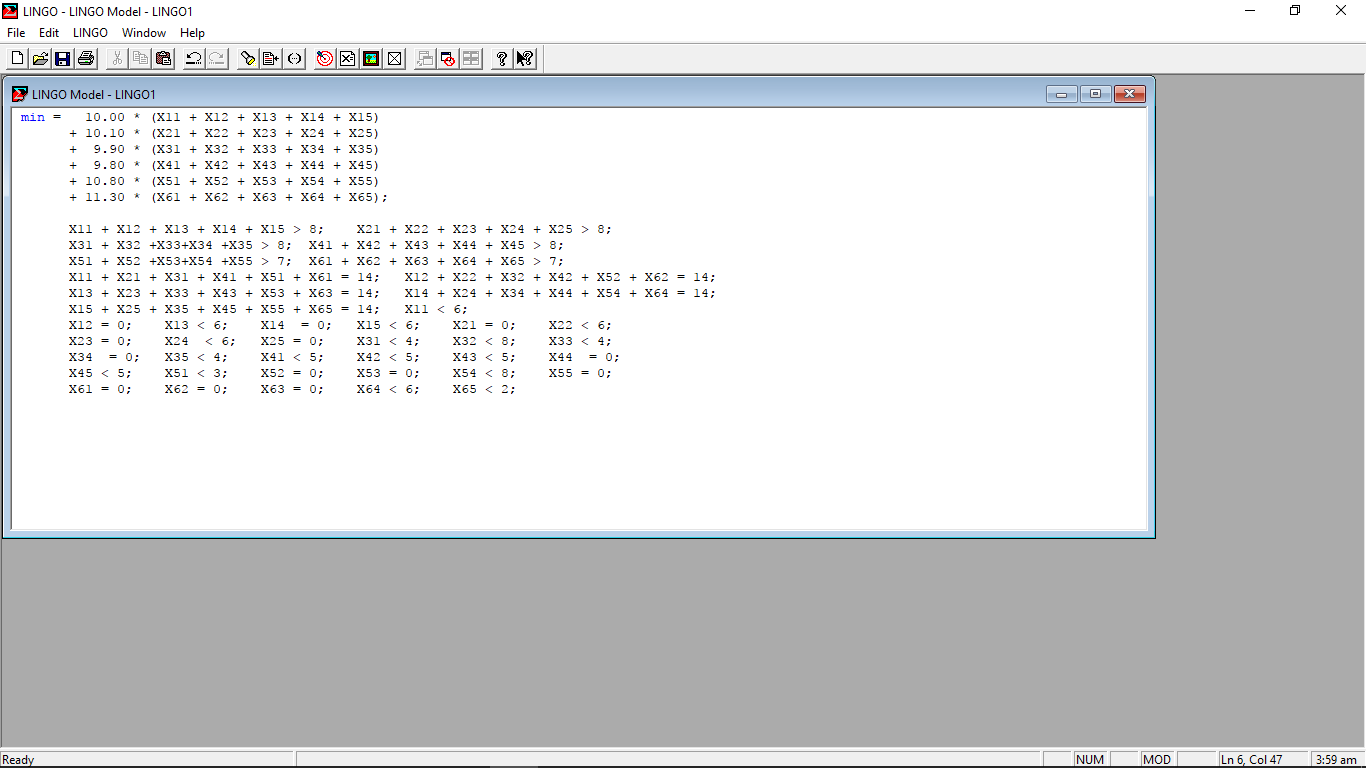
\includegraphics[width=0.9\textwidth]{81}
\end{frame}
\begin{frame}[fragile]{Solución LINGO}
    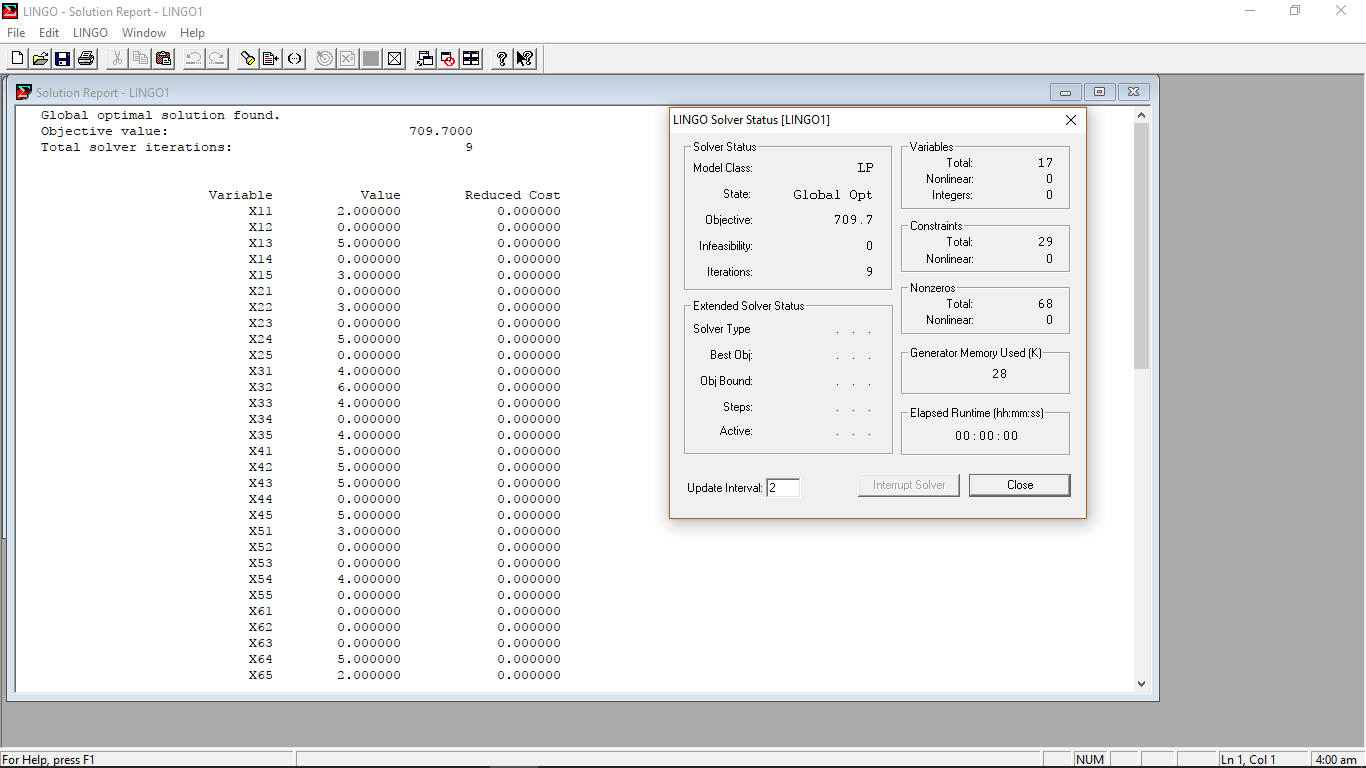
\includegraphics[width=0.9\textwidth]{82}
\end{frame}
\begin{frame}[fragile]{Solución LINGO}
    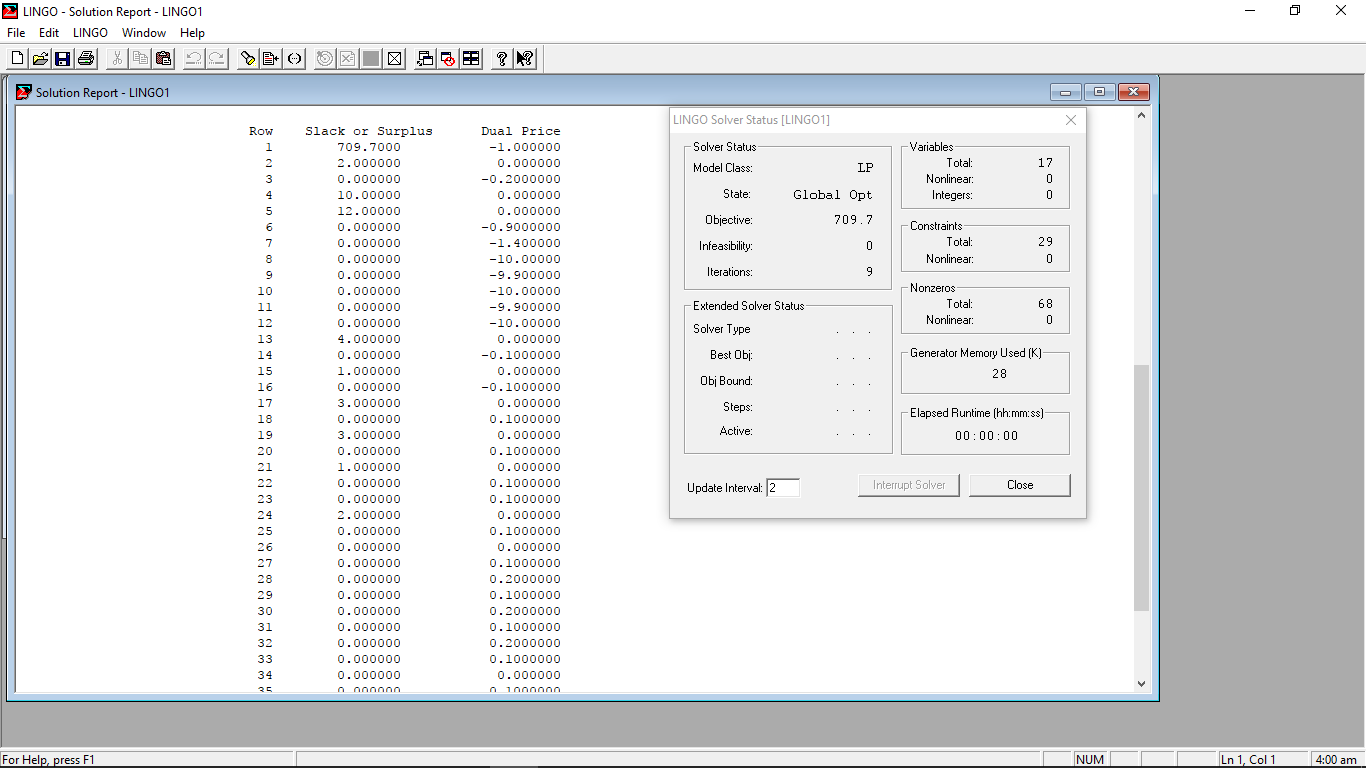
\includegraphics[width=0.9\textwidth]{83}
\end{frame}
\begin{frame}[fragile]{Solución LINGO}
    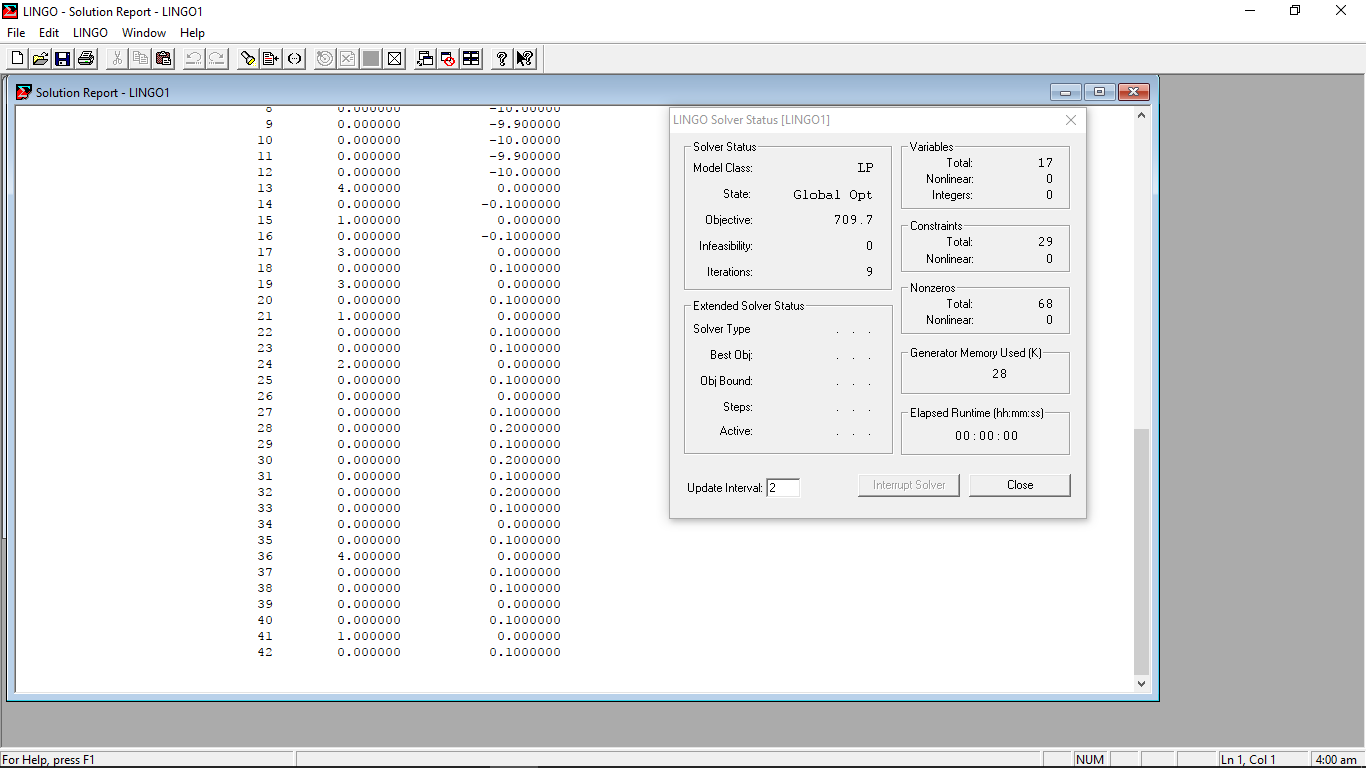
\includegraphics[width=0.9\textwidth]{84}
\end{frame}

\begin{frame}[fragile]{Solución Final}
\[Z = 709.7000 \]
\[X_{11} = 2\]
\[X_{12} = 0\]
\[X_{13} = 5\]
\[X_{14} = 0\]
\[X_{15} = 3\]
\[X_{21} = 0\]
\[X_{22} = 3\]
\[X_{23} = 0\]
\[X_{24} = 5\]
\end{frame}
\begin{frame}[fragile]{Solución Final}
\[X_{25} = 0\]
\[X_{31} = 4\]
\[X_{32} = 6\]
\[X_{33} = 4\]
\[X_{34} = 0\]
\[X_{35} = 4\]
\[X_{41} = 5\]
\[X_{42} = 5\]
\[X_{43} = 5\]
\end{frame}
\begin{frame}[fragile]{Solución Final}
\[X_{44} = 0\]
\[X_{45} = 5\]
\[X_{51} = 3\]
\[X_{52} = 0\]
\[X_{53} = 0\]
\[X_{53} = 4\]
\[X_{54} = 0\]
\[X_{55} = 0\]
\[X_{61} = 0\]
\end{frame}
\begin{frame}[fragile]{Solución Final}
\[X_{62} = 0\]
\[X_{63} = 0\]
\[X_{64} = 5\]
\[X_{65} = 2\]
\end{frame}

%Problema 9
\begin{frame}[t,fragile]{Problema 3.4-15 }
Joyce y Marvin tienen una guardería. \begin{wrapfigure}{r}{0.20\textwidth}
    \centering
    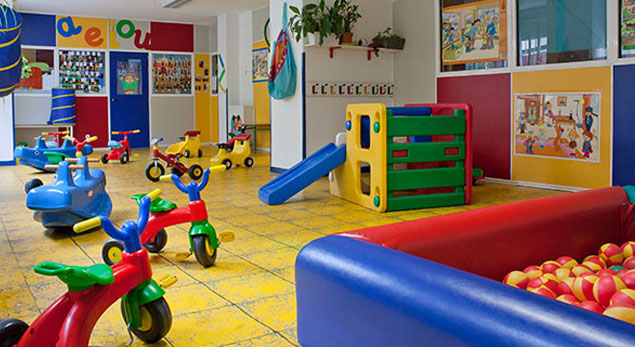
\includegraphics[width=0.20\textwidth]{9}
\end{wrapfigure} Ellos intentan decidir qué dar a los niños de almuerzo. Desean mantener costos bajos, pero también deben cumplir los requerimientos nutritivos para niños. Ya decidieron darles sándwiches de mantequilla de maní y mermelada  y alguna combinación de galletas, leche y jugo de naranja.El contenido nutritivo de cada alimento y su costo se presenta en la siguiente tabla:\\
\end{frame}
\begin{frame}[t,fragile]{Problema 3.4-15 }
\begin{tabular}{|c|c|c|c|c|c|}
\hline 
Alimento & Grasa & Total & Vit.C(mg) & Proteínas & Costo(\$) \\ 
\hline 
Pan& 10 & 70 & 0 & 3 & 5 \\ 
\hline 
Mantequilla de maní& 75 & 100 & 0 & 4 & 4 \\ 
\hline 
Galleta  & 20 & 60 & 0 & 1 & 8 \\ 
\hline 
Mermelada  & 0 & 50 & 3 & 0 & 7 \\ 
\hline 
Leche  & 70 & 150 & 2 & 8 & 15 \\ 
\hline 
Jugo  & 0 & 100 & 120 & 1 & 35 \\ 
\hline 
\end{tabular}
\end{frame}

\begin{frame}[t,fragile]{Problema 3.4-15 }
Los requerimientos nutritivos son los siguientes. Cada niño debe recibir de 400 a 600 calorías. No más de 30\% de las calorías totales debe venir en grasas. Cada niño debe consumir al menos 60 mg de vitamina C y 12 g de proteína. Todavía más, por razones prácticas, cada niño necesita justo 2 rebanadas de pan (para un sandwich), al menos el doble de mantequilla de maní que de mermelada y al menos una taza de líquido (leche y/o jugo de naranja). 
Joyce y Marvin desean seleccionar las opciones de alimento para cada niño que minimice el costo mientras cumple con los requerimientos establecidos.
\end{frame}
\begin{frame}[fragile]{Análisis}
Se requiere cubrir los requerimientos de la forma más barata posible. Como en el problema de la dieta visto en clases.

\end{frame}
\begin{frame}[fragile]{Variables de Decisión}
\[x_{1} = Rebanadas de pan\]
\[x_{2} = Cucharadas de mantequillas de maní\]
\[X_{3} = Cucharadas de fresa de mermelada\]
\[X_{4} = Unidades de Galletas integrales\]
\[X_{5} = Tazas de leche\]
\[X_{6} = Tazas de jugo\]

\end{frame}

\begin{frame}[fragile]{Función Objetivo}
Minimizar\\
\[Z = 5x_{1} + 4x_{2} +7X_{3} + 8X_{4} + 15X_{5} +36X_{6}\]
\end{frame}

\begin{frame}[fragile]{Restricciones}
Calorías mínimas:\\
\[70x_{1} + 100x_{2} + 50x_{3} + 60x_{4} + 150x_{5} + 100x_{6} >= 400\]
Calorías máximas:
\[70x_{1} + 100x_{2} + 50x_{3} + 60x_{4} + 150x_{5} + 100x_{6} <= 600\]
Grasa:\\
\[-11x_{1} + 45x_{2} - 15x_{3} + 2x_{4} + 25x_{5} - 30x_{6}  <=  0\]
Vitamina C:\\
\[3x_{3} + 2x_{5} + 120x_{6} >= 60\]
\end{frame}
\begin{frame}[fragile]{Restricciones}
Proteínas:\\
\[3x_{1} + 4x_{2} + x_{4} + 8x_{5} + x_{6} >= 12\]
Pan:
\[x_{1} = 2\]
Doble mantequilla de maní que mermelada:\\
\[x_{2} - 2x_{3} >= 0\]
Líquidos:\\
\[x_{5} + x_{6} >= 1 \]
Triviales\\
 \[x_{1}, x_{2}, x_{3}, x_{4}, x_{5}, x_{6} >= 0\]

\end{frame}

\begin{frame}[fragile]{Modelo Completo}
Minimizar\\
\[Z = 5X_{1} + 4X_{2} +7X_{3} + 8X_{4} + 15X_{5} +36X_{6}\]
Sujeto a :\\
\[70x_{1} + 100x_{2} + 50x_{3} + 60x_{4} + 150x_{5} + 100x_{6} >= 400\]
\[70x_{1} + 100x_{2} + 50x_{3} + 60x_{4} + 150x_{5} + 100x_{6} <= 600\]
\[-11x_{1} + 45x_{2} - 15x_{3} + 2x_{4} + 25x_{5} - 30x_{6}  <=  0\]
\[3x_{3} + 2x_{5} + 120x_{6} >= 60\]
\[3x_{1} + 4x_{2} + x_{4} + 8x_{5} + x_{6} >= 12\]
\[x{1} = 2\]
\[x_{2} - 2x_{3} >= 0\]
\[x_{5} + x_{6} >= 1 \]
\[x_{1}, x_{2}, x_{3}, x_{4}, x_{5}, x_{6} >= 0\]

\end{frame}

\begin{frame}[fragile]{Solución LINGO}
    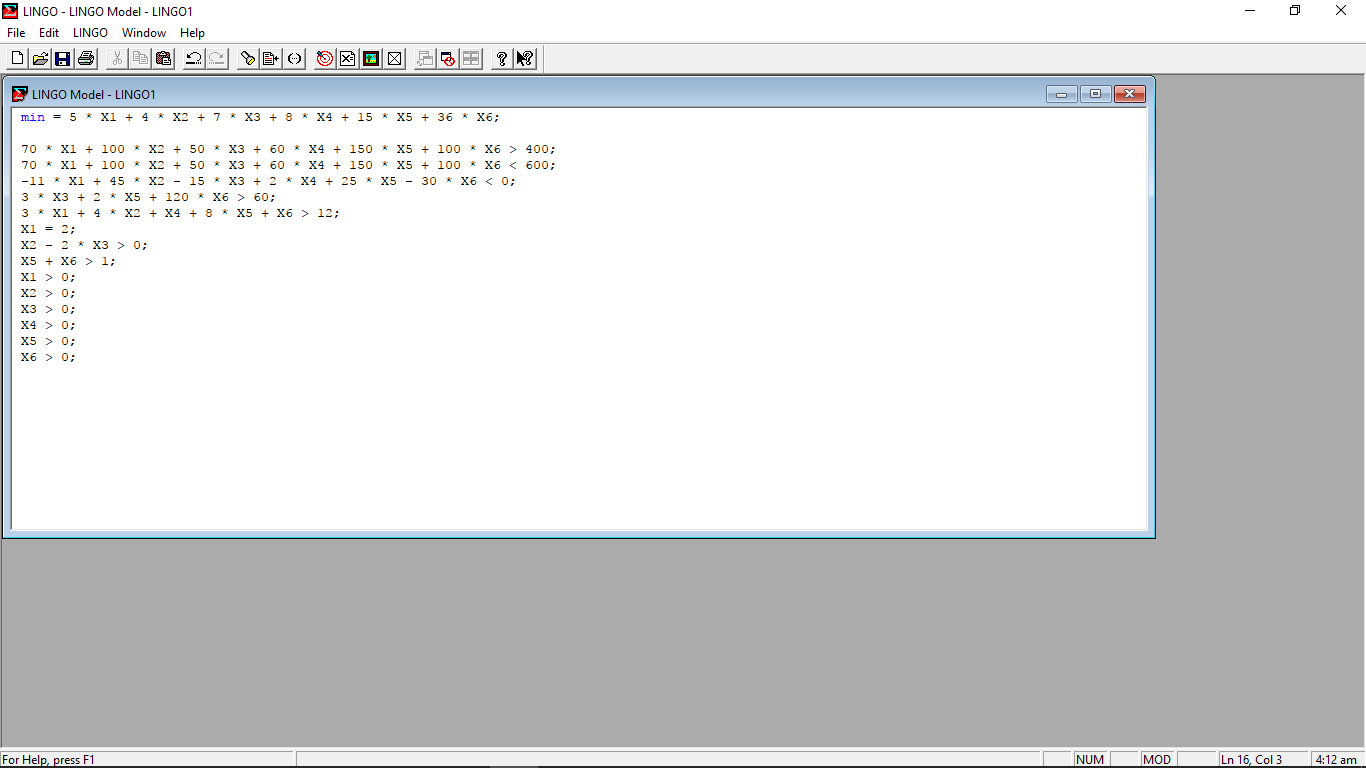
\includegraphics[width=0.9\textwidth]{92}
\end{frame}
\begin{frame}[fragile]{Solución LINGO}
    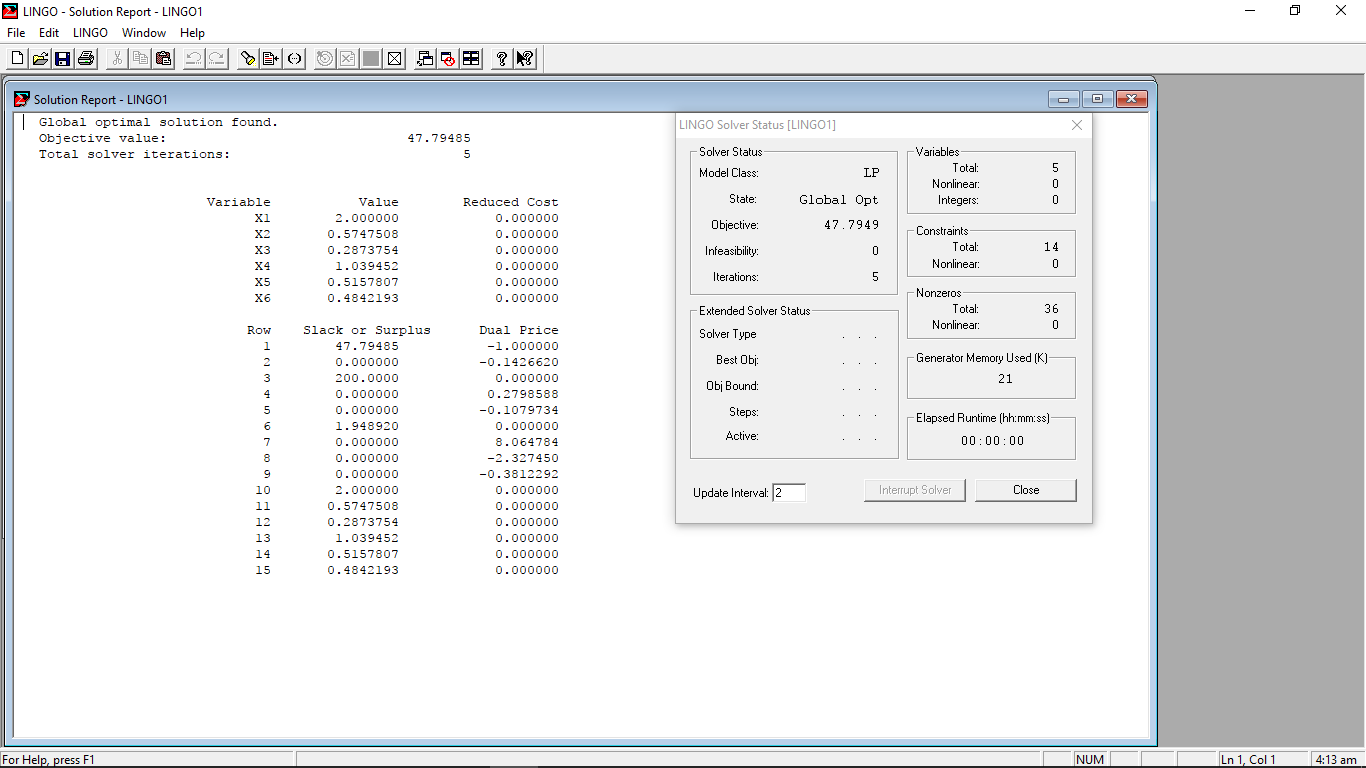
\includegraphics[width=0.9\textwidth]{91}
\end{frame}

\begin{frame}[fragile]{Solución Final}
\[Z = 47.79485 \]
\[X_{1} = 2.0000\]
\[X_{2} = 0.5747508\]
\[X_{3} = 0.2873754\]
\[X_{4} = 1.039452\]
\[X_{5} = 0.5157807\]
\[X_{6} = 0.4842193\]
\end{frame}

%Problema 10
\begin{frame}[t,fragile]{Problema 3.6-5 }
Maureen Laird es directora de inversiones de Alva Electric Co., empresa importante en el medio oeste. La compañía ha programado la construcción de nuevas plantas hidroeléctricas a 5, 10, y 20 años, para satisfacer las necesidades de la creciente población en la región servida por la empresa. Para cubrir por lo menos los costos de construcción, Maureen tiene que invertir parte del dinero de  la empresa para cubrir estas necesidades futuras de liquidez. Maureen Sólo puede comprar tres tipos de activos financieros, cada uno  cuesta \$ 1 millón por unidad.
 \begin{wrapfigure}{r}{0.20\textwidth}
    \centering
    
\includegraphics[width=0.20\textwidth]{10}
\end{wrapfigure}\\
\end{frame}

\begin{frame}[t,fragile]{Problema 3.6-5 }
Unidades fraccionarias pueden ser comprados. Los activos que produzcan ingresos de 5, 10 y 20 años a partir de ahora, y que los ingresos se necesitan para cubrir al menos el flujo de efectivo mínimo las necesidades de estos años. (Cualquier excedente de ingresos por encima del mínimo obligación de que cada período de tiempo se aprovechará para aumentar el pago de dividendos a los accionistas en lugar de guardarlo para ayudar a cumplir con el requisito mínimo de liquidez en el próximo período de tiempo.)La siguiente tabla muestra  los ingresos generados por cada unidad de cada activo y el  mínimo de ingresos necesarios para cada uno de los periodos futuros cuando una nueva central hidroeléctrica se construirá.
\end{frame}
\begin{frame}[t,fragile]{Problema 3.6-5 }
table
\end{frame}
\begin{frame}[t,fragile]{Problema 3.6-5 }
Maureen desea determinar la mezcla de inversiones en estas acciones que cubrirá los requerimientos de efectivo y que minimizará la cantidad total invertida.
\end{frame}

\begin{frame}[fragile]{Análisis}
Se quiere determinar la mezcla de inversiones  para las acciones, que cumplan con los requerimientos  y que minimice la cantidad total invertida, que sea el óptimo. Es decir, que me diga la cantidad que debo invertir en el activo 1, cuánto debo invertir en el activo 2 y cuánto debo invertir en el activo 3.

\end{frame}

\begin{frame}[fragile]{Variables de Decisión}
\[X_{1} = La cantidad de inversión para el activo 1\]
\[X_{2} = La cantidad de inversión para el activo 2\]
\[X_{3} = La cantidad de inversión para el activo 3\]

\end{frame}

\begin{frame}[fragile]{Función Objetivo}
Minimizar\\
\[Z = X_{1} + X_{2} + X_{3}\]
\end{frame}

\begin{frame}[fragile]{Restricciones}
\[2X_{1} + 2X_{2} +0.5X_{3}  >= 400\]
\[0.5X_{1} + 0.5X_{2} +X_{3} >= 100\]
\[1.5 X_{1} + 3X_{3} >= 300\]
\[X_{1}, X_{2}, X_{3} >= 0\]

\end{frame}

\begin{frame}[fragile]{Modelo Completo}
Minimizar:
\[Z = X_{1} + X_{2} + X_{3}\]
Sujeto a :\\
\[2X_{1} + X_{2} +0.5X_{3}  >= 400\]
\[0.5X_{1} + 0.5X_{2} +X_{3} >= 100\]
\[1.5 X_{2} + 2X_{3} >= 300\]
\[X_{1}, X_{2}, X_{3} >= 0\]

\end{frame}

\begin{frame}[fragile]{Solución LINGO}
    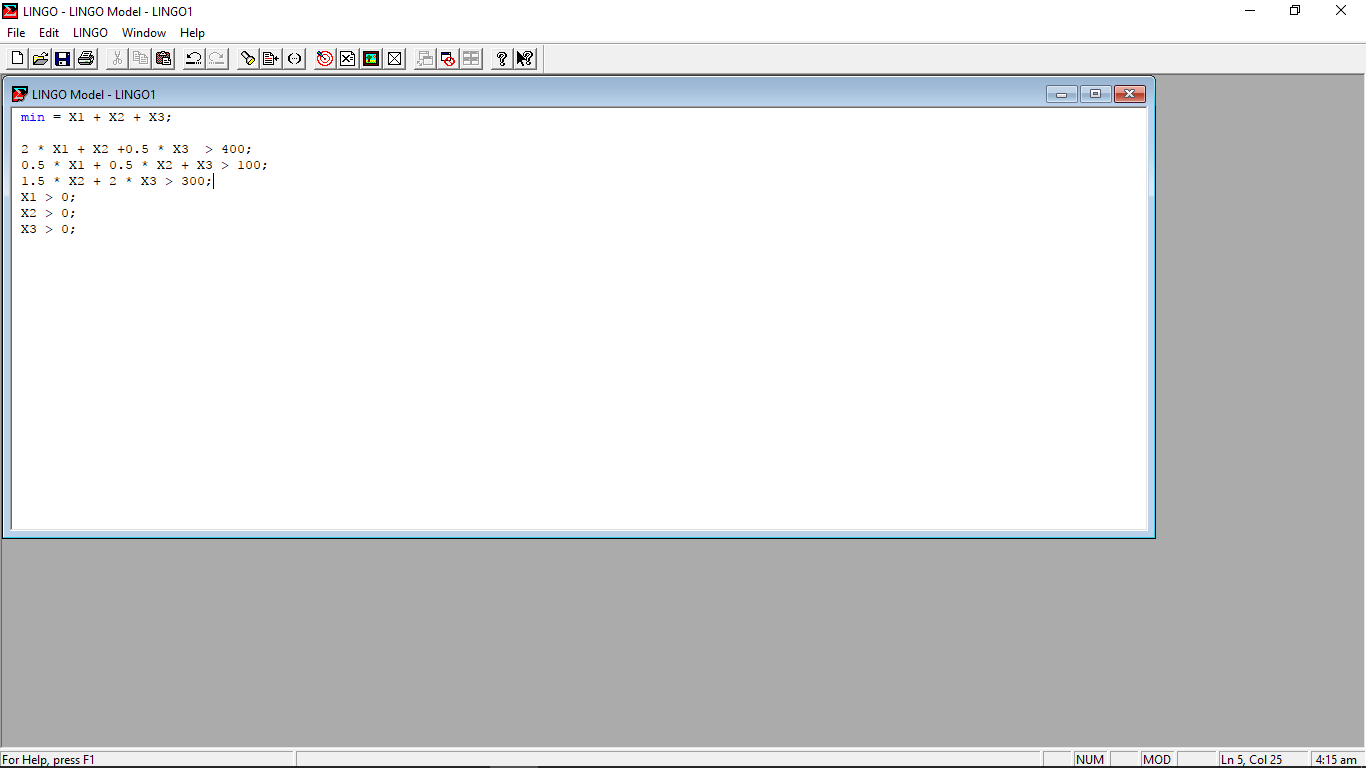
\includegraphics[width=0.9\textwidth]{102}
\end{frame}
\begin{frame}[fragile]{Solución LINGO}
    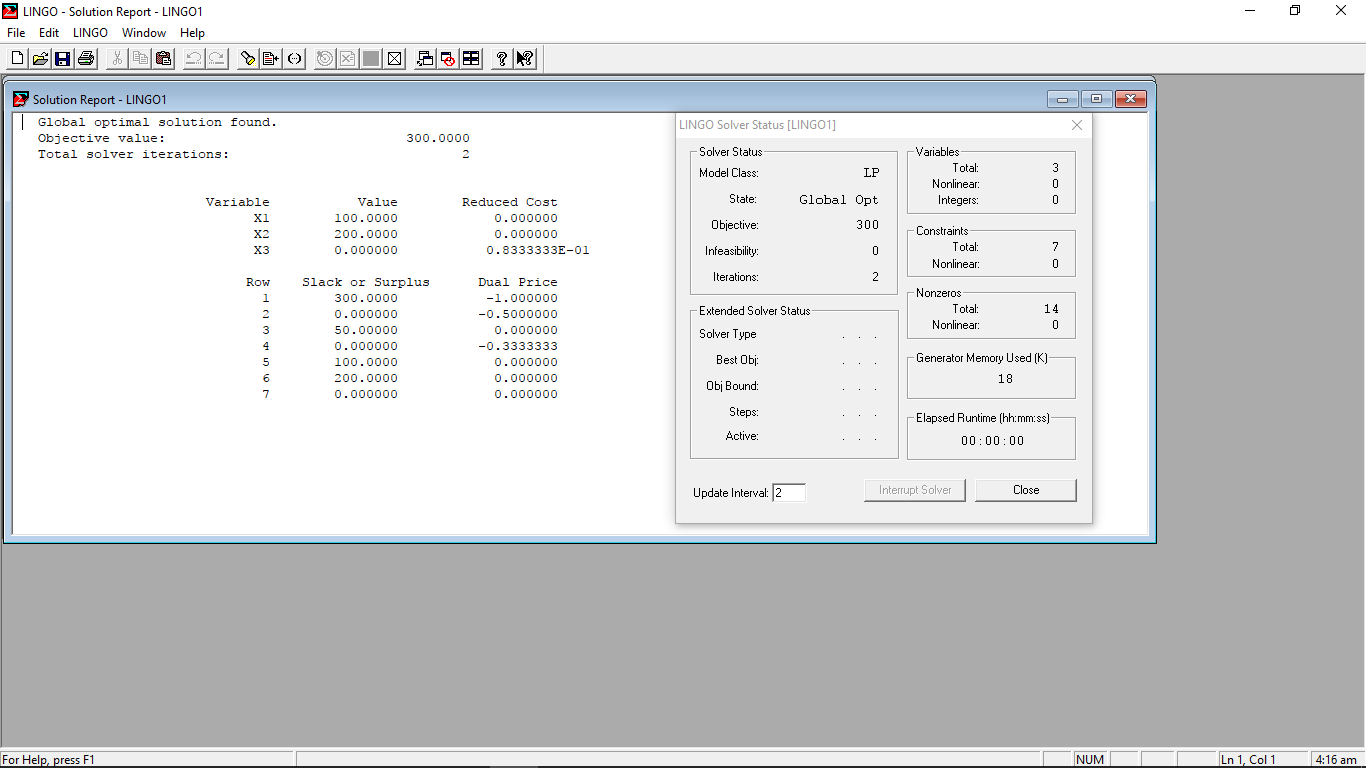
\includegraphics[width=0.9\textwidth]{101}
\end{frame}

\begin{frame}[fragile]{Solución Final}
\[Z = 300.0000\]
\[X_{1} = 100.0000\]
\[X_{2} = 200.0000\]
\[X_{3} = 0.0000\]
\end{frame}

\end{document}
%\tikzmarkin<1>{b}y\tikzmarkend{b}
